%%%%%%%%%%%%%%%%%%%%%%%%%%%%%%%%%%%%%%%% Klasse Festlegen
%\documentclass[Master,BMR,english]{BASE/twbook}
\documentclass[Bachelor, BIC, english, fhCitStyle, IEEE]{BASE/twbook} % FH definierte Zitierstandards verwenden
%%%%%%%%%%%%%%%%%%%%%%%%%%%%%%%%%%%%%%%% Verwendete Packages
\usepackage[utf8]{inputenc} % Zeichen-Enkodierung (evtl. Abweichungen für Apple)
\usepackage[T1]{fontenc} % Zeichen-Enkodierung
\usepackage{blindtext} % Platzhaltertexte
\usepackage{minted} % Darstellung von Code
\usepackage{comment} % Auskommentieren von ganzen Passagen
\usepackage{csquotes}
\usepackage{algorithm} % Umgebung f Algorithmen
\usepackage[noend]{algpseudocode}
% Wenn Sie während Ihrer Arbeit
% merken, dass Sie zusätzliche Funktionen
% benötigen ist hier ein guter Platz um
% weitere Packages zu laden
\usepackage{svg}
\usepackage{mdframed}
\graphicspath{ {./PICs/} }
%%%%%%%%%%%%%%%%%%%%%%%%%%%%%%%%%%%%%%%% Zitierstil zum selbst definieren
\usepackage[backend=biber, style=ieee]{biblatex} % LaTeX definierter IEEE- Standard
%\usepackage[backend=biber, style=authoryear]{biblatex}      % LaTeX definierter Harvard-Standard
\addbibresource{Literature.bib} % Literatur-File definieren
%%%%%%%%%%%%%%%%%%%%%%%%%%%%%%%%%%%%%%%% Custom commands
% Redefine \section, \subsection, \subsubsection to not add entries to the ToC
% Define a command to temporarily disable \addcontentsline
\newcommand{\nocontentsline}[3]{}
% Define commands to create sections, subsections, and subsubsections without ToC entries
\newcommand{\hidsection}[1]{\bgroup\let\addcontentsline=\nocontentsline\section{#1}\egroup}
\newcommand{\hidsubsection}[1]{\bgroup\let\addcontentsline=\nocontentsline\subsection{#1}\egroup}
\newcommand{\hidsubsubsection}[1]{\bgroup\let\addcontentsline=\nocontentsline\subsubsection{#1}\egroup}
% Defines an alias for writing inline monospace font for code related things
\def\code#1{\texttt{#1}}
% src: https://tex.stackexchange.com/questions/194426/split-itemize-into-multiple-columns
\usepackage{etoolbox,refcount}
\usepackage{multicol}

\newcounter{countitems}
\newcounter{nextitemizecount}
\newcommand{\setupcountitems}{%
  \stepcounter{nextitemizecount}%
  \setcounter{countitems}{0}%
  \preto\item{\stepcounter{countitems}}%
}
\makeatletter
\newcommand{\computecountitems}{%
  \edef\@currentlabel{\number\c@countitems}%
  \label{countitems@\number\numexpr\value{nextitemizecount}-1\relax}%
}
\newcommand{\nextitemizecount}{%
  \getrefnumber{countitems@\number\c@nextitemizecount}%
}
\newcommand{\previtemizecount}{%
  \getrefnumber{countitems@\number\numexpr\value{nextitemizecount}-1\relax}%
}
\makeatother    
\newenvironment{AutoMultiColItemize}{%
\ifnumcomp{\nextitemizecount}{>}{3}{\begin{multicols}{2}}{}%
\setupcountitems\begin{itemize}}%
{\end{itemize}%
\unskip\computecountitems\ifnumcomp{\previtemizecount}{>}{3}{\end{multicols}}{}}
%%%%%%%%%%%%%%%%%%%%%%%%%%%%%%%%%%%%%%%% Einträge für Deckblatt
\title{Precision at Pixel-Level:\\\acl{yoloAlt} doing UI test automation}

\author{Nikolaus Rieder}
\studentnumber{2010258028}
%\author{Titel Vorname Name, Titel\and{}Titel Vorname Name, Titel}
%\studentnumber{XXXXXXXXXXXXXXX\and{}XXXXXXXXXXXXXXX}

\supervisor{Dr. Dietmar Millinger}
%\supervisor[Begutachter]{Titel Vorname Name, Titel}
%\supervisor[Begutachterin]{Titel Vorname Name, Titel}
%\secondsupervisor{Titel Vorname Name, Titel}
%\secondsupervisor[Begutachter]{Titel Vorname Name, Titel}
%\secondsupervisor[Begutachterinnen]{Titel Vorname Name, Titel}

\place{Wien}
%%%%%%%%%%%%%%%%%%%%%%%%%%%%%%%%%%%%%%%% Danksagung/Kurzfassung/Schlagworte
% Abstract
\outline{ Developing and executing test suites on embedded devices with a \ac{gui} can be a time-consuming and exhaustive process. Nevertheless, it is a necessary task in interfaces of critical infrastructure, like \ac{fas} or \ac{hcs} developed at Schrack Seconet. This research analyzes the viability of using machine learning for identifying and detecting \ac{ui} widgets based purely on screenshot data. The analysis is written from the perspective of \ac{ta} performed on critical systems like the aforementioned. The focus is on high performing results due to the qualitative requirements in \ac{ui} test automation of such systems, where upcoming problems during development are considered potentially critical if not detected. \\ During paper development, a \ac{yolo} model was trained on randomly synthesized datasets of \ac{ui} screenshots. The datasets were generated with the \ac{lvgl}, a common and popular library in embedded systems. During development of the datasets and model training processes, key problem factors are identified and potential mitigations addressed. The findings showcase these points in the context of a nurse call system, where reliability of the user interface plays a critical role and margin for error is non-existent. \\ The project follows a Design Science research approach, in which a \ac{ui} generator for \ac{lvgl} was created, that is capable of generating datasets of randomly chosen and placed widgets on a screen, as well as the generation of realistic looking designs by using a system based on a \ac{json} schema. In order to create larger datasets, a \ac{llm} was used to design multiple \ac{ui}s from a list of pre-defined contexts and themes. \\\\ This research aims to reduce time spent in test development and improve test coverage of varied \ac{ui}s in devices of critical systems, while aiding human developers in manual and automated testing. \\ }
\keywords{YOLOv8, UI Testing, embedded devices, widget detection, widget
classification, automated testing}
% Acknowledgements
\acknowledgements{I extend my gratitude to the faculty and staff at UAS Technikum Vienna for their invaluable guidance and the wealth of knowledge they have shared, which has culminated in the completion of this bachelor thesis. Special appreciation is given to my academic advisor, Dietmar Millinger, for his expertise and dedication. Additional thanks are due to Dietmar Millinger, Karl M. Göschka, Lorenz Froihofer, and Susanne Teschl for their inspiration and exceptional contributions to my understanding of machine learning, computer science, and mathematics, respectively. Thanks should also go to my academic peers, for the collaborative environment fostered on our student community server and the valuable networks we have built throughout this educational journey. I am particularly grateful to my partner, whose support and patience were unwavering during my academic endeavors at the UAS Technikum Vienna. I would also like to express my sincere thanks to Schrack Seconet AG for providing me with the opportunity to develop this paper in a professional context. The support from colleagues has been instrumental in aligning my academic pursuits with practical applications in the workplace. Lastly, I thank my own body and mind for not breaking apart throughout the long days and mostly nights that were involved up to this point.}
\setListingsAndAcronyms % Definition der Namen für Quellcodeverzeichnis
%%%%%%%%%%%%%%%%%%%%%%%%%%%%%%%%%%%%%%%%%%%%%%%%%%%%%%%%%%%%%% End of header
%%%%%%%%%%%%%%%%%%%%%%%%%%%%%%%%%%%%%%%%%%%%%%%%%%%%%%%%%%%%%% Start of document
\begin{document}
%%%%%%%%%%%%%%%%%%%%%%%%%%%%%%%%%%%%%%%% Title page in FHTW style
\maketitle
%%%%%%%%%%%%%%%%%%%%%%%%%%%%%%%%%%%%%%%%%%%%%%%%%%%%%%%%%%%%%% Start of content
%%%%%%%%%%%%%%%%%%%%%%%%%%%%%%%%%%%%%%%% Start of Introduction
\chapter{Introduction}
In embedded systems providing critical infrastructure, it is often mandatory to have well-established and good testing procedures. One such system is nurse call used in hospitals and health care facilities, which consists of devices that allow humans to call for help in situations ranging from mundane \textit{(e.g. requesting patient service)} to life-threatening \textit{(e.g. cardiac arrest alarm)} use-cases. These systems require interfaces for human interaction and such interfaces need to be rigorously tested, to provide feedback on system quality in early stages of development, where the potential for harm is very low. Additionally, automated testing becomes necessary, to reduce possible variation in test execution when compared to manual testing, where human-error is more prevalent than with machines repeating test cases.\\
However, when such interfaces only consist of a touch display, it can become very challenging to automate, as it requires tools for the machine to analyze the visual image and to interact with the \ac{ui} using stimuli \textit{(e.g. simulated touch)}. The automation gets further complicated, the more inputs and outputs the machine needs to deal with in order to perform a representative human test routine. Once such test routines are established, they need to be continously maintained in order to adapt to changes to the \ac{ui}, otherwise such changes can break the test system and halt the overall development process.\\
This research project will demonstrate a machine learning tool to aid in analyzing images to obtain metadata about the displayed \ac{ui}. The metadata consists of position and size of individual widgets, which then can be used in testing routines for precise functional interactions. By training a model that can detect and classify widgets based on screenshots, the testing routines can adapt to many \ac{ui} arrangements dynamically, which can reduce labor involved for maintenance of test repositories.\\
Since covering all possible \ac{ui} libraries and frameworks would be tremendous in scope, the research will limit focus on \ac{lvgl} as the basis for the \ac{ui}. It begins by creating an image and annotation generator for \ac{lvgl}, since there is no available dataset for this library specifically and it also allows for targeted adjustments in dataset size, variation and balance of widget types. Furthermore, it allows for validation based on a real world example from the company where the author is employed at. The work will also be limited to a subset of available widget types, to provide a basic baseline for the viability of the tool, which may be easily extended in the future.\\
Once dataset creation is automated, the paper will demonstrate training based on the \ac{yolo} model and evaluate performance in comparison to human methods. From a testing perspective, this paper is most concerned with the prediction accuracy of the model, since a tool that is not capable of reliable detection will only shift maintenance problems to the tool itself, rather than improving them overall.
%%%%%%%%%%%%%%%%%%%%%%%%%%%%%%%%%%%%%%%%%%%%%%%%%%%%%%%%%%%%%%%%%%
\clearpage
%%%%%%%%%%%%%%%%%%%%%%%%%%%%%%%%%%%%%%%% Start of Problem description
\chapter{Problem description}
When developing automated test cases for a product which has very long life cycles, due to being incorporated in building infrastructure for 10 years or more, it can be expected that involved maintenance labor of existing test cases surpasses the creation of new test cases. But even in such long-lasting products, big system changes \textit{(e.g. \ac{ui} redesign, new controller architecture, new graphics libraries...)} eventually occur. Such a change incurs a new evaluation and design of existing test procedures, to accommodate for the new system or \ac{ui}, even if the actual use-case and performed steps fundamentally remain the same.
For the business it is therefor beneficial to have testing tools, which reduce the maintenance costs of such legacy test costs, by being dynamic and adaptable to the given test environment.\\
% THIS PART requires more research in the literature to write a more coherent problem description
% I DON'T EVEN KNOW IF I NEED THIS PART
% Such a change incurs a new evaluation and design of existing test procedures, to accommodate for the new system or \ac{ui}, even if the actual use-case and performed steps fundamentally remain the same. The development of a breaking change must then factor in the costs of changing legacy tests and it may result in decisions that will have less test quality as a result, in favor of bringing in more money for the business.\\
% Therefor it can be beneficial for the tester to make use of tools, which reduce development costs incurred.
% When developing test cases for \aclp{ui}, it is necessary to differentiate between white-box and black-box testing. A white-box testing approach would incorporate knowledge about the code of the \ac{ui}, where a tester would know about the types of widgets used and their applied properties, amongst other things related to the contents of the source. This testing approach is typically used in unit and early integration testing, possibly performed by the developer themselves. In black-box testing, such information is completely stripped away and it is best-practice to leave such work to people outside of the development team to avoid confirmation-bias. % TODO citations for testing approaches, best-practice, etc.
% The context of this paper focuses on the latter with the limitation, that the author has knowledge of the library used and the hardware product itself. The author is a professional in testing and test automation, aware of the risks involved when it comes to knowledge about inner workings of the system under test. % TODO citation of involved risks due to confirmation bias
% As such, the main input for the tool will be limited to what is accessible to the tester, which is constrained to be a black-box testing approach.\\
\section{Problem context at Schrack Seconet}
New developed products by Schrack Seconet will use the \acf{lvgl} \autocite{LVGLLightVersatile}, a popular choice in embedded hardware for developing user interfaces. This framework already comes with implementations that allow for simulation of the \ac{ui} rendering on a development machine, which already improves development time since it doesn't require display hardware to develop and test \ac{ui} design.
But being a library targeted at embedded systems, there are no integrated testing tools that would allow a test automation developer to verify the functionality of those designs on the actual hardware. The nurse call system \ac{vcip} \autocite{VisocallIPModerne} is a distributed embedded system, which relies on multiple hardware devices to interact with each other and \ac{ui} functionality is tied to the signals and messages of the system as a whole.
When it comes to simulation, it marks unit testing of the user interface as an unusable solution, due to the inherent complexity of the system and the required simulation of multiple devices or peripherals for the \ac{ui} to function properly.\\
Instead, the developers at Schrack Seconet integrated a low-level kernel \ac{api} into the development firmware of \ac{ui} devices, which allows for simulation of user interactions on the devices, mimicking human behavior on the display. The mimicked behavior includes interactions such as touch, press, release, drag and combined variations of the aforementioned.\\
However, this approach requires knowledge about the metadata of the \ac{ui} by the test developer, so that the defined interactions are performed on the correct coordinates of the user interface element.\\
A common example of such a test case using coordinates is visible in Fig.\ref{fig:lock-screen-test-example}, showing a routine which unlocks the screen by swiping.
\begin{figure}
    \caption{Example of a lock screen test case using absolute coordinates by Schrack Seconet}
    \centering
    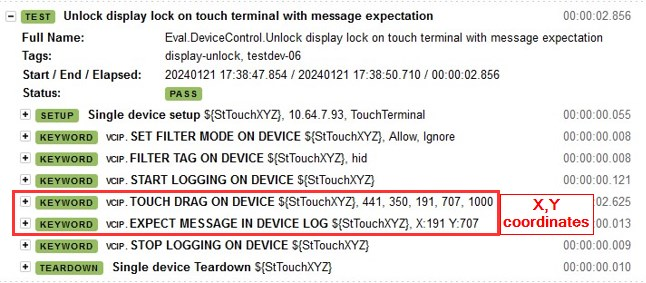
\includegraphics[width=\textwidth]{lock-screen-testcase.jpg}
    \label{fig:lock-screen-test-example}
\end{figure}\\
Expected functionality of the device is then assessed by aggregation of device logging data, verification of expected signal states from accessible hardware outputs. These outputs typically are \acp{led} on the test device itself or other interconnected devices in the distributed system, which are connected through proprietary IP-based protocols or other proprietary hardware bus technologies employed by the Schrack Seconet system. In addition to these expectations, the raw frame buffer of the controller can be exported to the test machine, which will also depict any visual errors, as long as the error occurred in firmware and not during transmission to the display driver. An example of such a visual error is depicted in Fig.\ref{fig:visual-error-example-screendump}.
\begin{figure}
    \caption{Example of a visual error on the lock screen of a \ac{vcip} product in development}
    \centering
    
\includegraphics[height=0.25\textheight]{screen_dump_error.png}
    \label{fig:visual-error-example-screendump}
\end{figure}
\newpage
\hidsubsubsection{Demand for new testing methods}
The current approach works well for a given user interface design which is not affected by frequent changes, but we currently lack in verification on the visual aspect of the user interface itself. Furthermore, it comes with an inherent problem in maintenance and development time, since the test automation engineer is required to determine the element coordinates through reverse engineering or by inspecting the firmware code-base.\\
The latter approach is generally frowned upon in the company, as we prefer a tendency towards black-box-testing, which mitigates the chance of overlooking software bugs due to code blindness. It is preferred for the test automation engineer to have as little knowledge about the implementation of the firmware as possible, so that the tester can focus on unbiased verification of the target device.
It also would not be a viable approach to look through the codebase to determine the element coordinates, since it typically is not blatantly written inside the code and would require the tester to work through the programmatic abstractions.
\\
Coordinates of \ac{ui} elements are typically reverse engineered by inspecting screen dumps from the test device itself. The generated image file has the exact dimensions as the device display, and it is easy to determine coordinates through generally available image viewers, such as IrfanView \autocite{IrfanViewOfficialHomepage}. The positions of \ac{ui} elements is then embedded into automated test case routines, which will perform the defined \ac{ui} interactions. Functional expectations are then verified through existing test framework capabilities.\\
This approach comes with a caveat, as the hard-coded metadata is bound to become invalid when \ac{ui} changes, like when new products are developed as previously mentioned. This results in a rework of all affected test cases. This can be mitigated through abstractions (e.g. global variables, re-usable routines), but ultimately remains a very labor-intensive maintenance process due to the sheer amount of individual coordinates for specific elements and menus.
\\
Another perspective on the current approach is the existing dependency on manual testing, since the described test method does not involve visual verification. The existing test automation can reliably assess the correct execution of functions in the system, but is incapable of finding errors that exist in the displayed image and animation on the device itself. The visual aspect of the \ac{ui} plays an important in nurse call systems, since it involves multiple languages for text, standards for visual and acoustic signalization described in the VDE-0834 \autocite{DINVDE08341}, and also the visual prioritization of emergency calls.
\\
Making use of the aforementioned screen dumps to assess these visual aspects would be a valid approach, but this has not been done so far and through this paper the development on a solution began. This visual verification however would still not account for errors that happen between transmission from the \ac{mcu} frame buffer to the display driver chip, but that is a negligible error source.
\\
A solution, which is capable of dealing with the dynamic nature of user interfaces, visual verification and future \ac{ui} development changes is highly sought after in the company. Computer vision and machine learning is assumed to be a promising approach for the purpose of reducing the cost and time involved in manual and automatic testing of these user interfaces.
\clearpage
%%%%%%%%%%%%%%%%%%%%%%%%%%%%%%%%%%%%%%%% Start of research questions
\chapter{Research questions}
\begin{itemize}
    \item \textbf{Is YOLOv8 a viable model for detecting \ac{lvgl} widgets based on screenshots?}\\
    In order for a model to be viable in widget detection for the previously stated problem context of test automation, it would need to have a high prediction confidence with accurate results. If the selected model fails to perform well, it will only bring rise to many false-positives when performing test routines, ultimately failing adoption and qualitative trust in the tool. The exact target accuracy to overcome was not possible to determine, as humans can make errors in writing coordinates and given how minor these incidents are, they are generally not documented. But given the critical context of the \ac{sut} a general approximation of minimum 80\% confidence and accuracy seems like a fair target. This number was chosen out of experience, as the remaining 20\% error margin would be manageable with review processes of the model output, as it is already the case for test case development.
    \item \textbf{Can \ac{ml} be a viable tool in aiding test developers through automatic widget localization?}\\
    In order for the \ac{ml} tool to properly aid the developer, it would need to make the general test development process faster and provide automation. Since the purpose of the tool is to provide coordinate metadata and the current process involves acquiring this information manually per single image, it would already be viable enough if the tool could automate this behaviour over a given set of images and return the desired coordinates. An additional step could also take care of integrating the detection into test routines themselves and performing the localization live, however that integration is out-of-scope for the paper itself.
\end{itemize}
It was considered to answer these questions for the ongoing development of a new \ac{ui} design at the company, however the release planning and starting time for that development did not correlate well with the thesis deadline. The answers to these questions will therefor be written based on the results of the synthesized data.
\clearpage
%%%%%%%%%%%%%%%%%%%%%%%%%%%%%%%%%%%%%%%% Start of literature & theory
\chapter{Existing literature and theoretical basis}
The topic of the thesis is specific to applying a \ac{ml} based object detection model for acquiring coordinate metadata of \ac{ui} elements, to be used in \ac{vgt} on devices of a distributed embedded systems. A direct comparison in that regard has not been found at the time of writing. But the comprehensive survey \autocite{garousiTestingEmbeddedSoftware2018} on embedded systems testing serves as a good start for systematic approaches.\\
In an article \autocite{linImprovingAccuracyAutomated2014}, the method of using record-and-play is described, with the goal of improving test accuracy. It uses the display data sent to a host PC and analyzes events performed by a manual tester to record test cases. In another step, the recorded events are played back to the device. However, this approach is not very easy to perform on distributed embedded systems, with various displays involved. It also comes with a performance challenge and the cost of proprietary technologies used.\\
In the field of mobile applications, a few studies were made using ML models to perform testing or create metadata of the graphical model of the UI. (i.e. element types, hierarchical structure, detection and recognition, state) \autocite{altinbasGUIElementDetection2022,chengMobileApplicationGUI2021,liWidgetCaptioningGenerating2020,selcukComparisonYOLOv5YOLOv82023,zhangDeepLearningBasedMobile2020,zhangMachineVisionbasedTesting2022, cavsakCavsakGUIComponent} A common dataset used in these studies is the RICO dataset \autocite{dekaRicoMobileApp2017}.
These studies share similarities of the upcoming research in regard to their usage of a \ac{ml} model for gathering metadata about \ac{ui}. Notably their software applications and user interfaces typically are written in languages and frameworks with better tooling support for performing visual automated testing.\\
An interesting case was made with the AI-driven tool "Owl Eye" \autocite{gamalOwlEyeAIDriven2023}, which can detect visual defects or inconsistencies in graphical user interface, based purely on provided screenshots. Two models, Faster-RCNN and \ac{yolo8}, were trained on the RICO dataset, with a concluding choice on \ac{yolo8} due to higher accuracy and faster training time. The choice of model for this thesis was inspired by the results showcased in that paper.\\
These aforementioned studies hint towards a possible improvement through the usage of ML for visual testing and also the general improvement of quality, due to performing better than manual testing. As such, the thesis will explore if \ac{ml} object detection is a viable and also reliable tool to aid in test development requiring coordinate metadata of \ac{ui} elements.
\newpage
\hidsection{\acf{cnn}}
\acp{cnn} are a type of deep neural networks, which are predominantly used for analyzing visual data. Resulting models have showcased remarkable success in various computer vision tasks, with the possibly fastest currently being the \ac{yolo} model. It was originally developed and researched by Joseph Redmon \autocite{redmonYouOnlyLook2016}, but has since seen multiple version updates, with one of the latest being \ac{yolo8} \autocite{jocherUltralyticsYOLO2023}.\\
The core idea behind \acp{cnn} is to learn spatial hierarchies of features from input images through the usage of convolution layers, meaning the underlying mathematical foundation is to perform convolution operations.\\
A \ac{cnn} typically consists of several layer types:
\begin{itemize}
    \item Convolution layers, which apply a set of convolution filters to the input image to capture local patterns (i.e. edges, textures, shapes)
    \item Pooling layers, which reduce the spatial dimensions of the input. This helps in reducing computational load and controlling over fitting. Common techniques include max pooling and average pooling.
    \item Fully connected layers, which are traditional neural networks typically placed at the end to perform the high-level reasoning based on the extracted features.
\end{itemize}
\hidsubsection{\acf{yolo} architecture}
The \ac{yolo} model architecture is a family of single-shot object detectors. They are known for their efficiency, due to their bounding box and class probability predictions performed directly on full images in a single evaluation. The single evaluation is also what gave the well-known model name "You only look once".\\
The architecture of the \ac{yolo8} model, further visualized in Fig.\ref{fig:yolov8-model-architecture}, consists of two main parts:
\begin{itemize}
    \item \textbf{Backbone}\\
    The backbone is responsible for extracting features from a given input image. It contains series of convolution layers, as well as further operations to down sample the image and  capture the spatial hierarchies of features.
    \item \textbf{Head}\\
    The head processes features extracted by the backbone and is responsible for predicting the bounding boxes and class probabilities. A detection layer refines the feature maps and will predict the object locations and classes at multiple image scales.
\end{itemize}
Further details about the architecture can be determined through the open-source repository of the model \autocite{jocherUltralyticsYOLO2023}.
\begin{figure}
    \caption{Model structure of YOLOv8 detection models by RangeKing \autocite{BriefSummaryYOLOv8}}
    \centering
    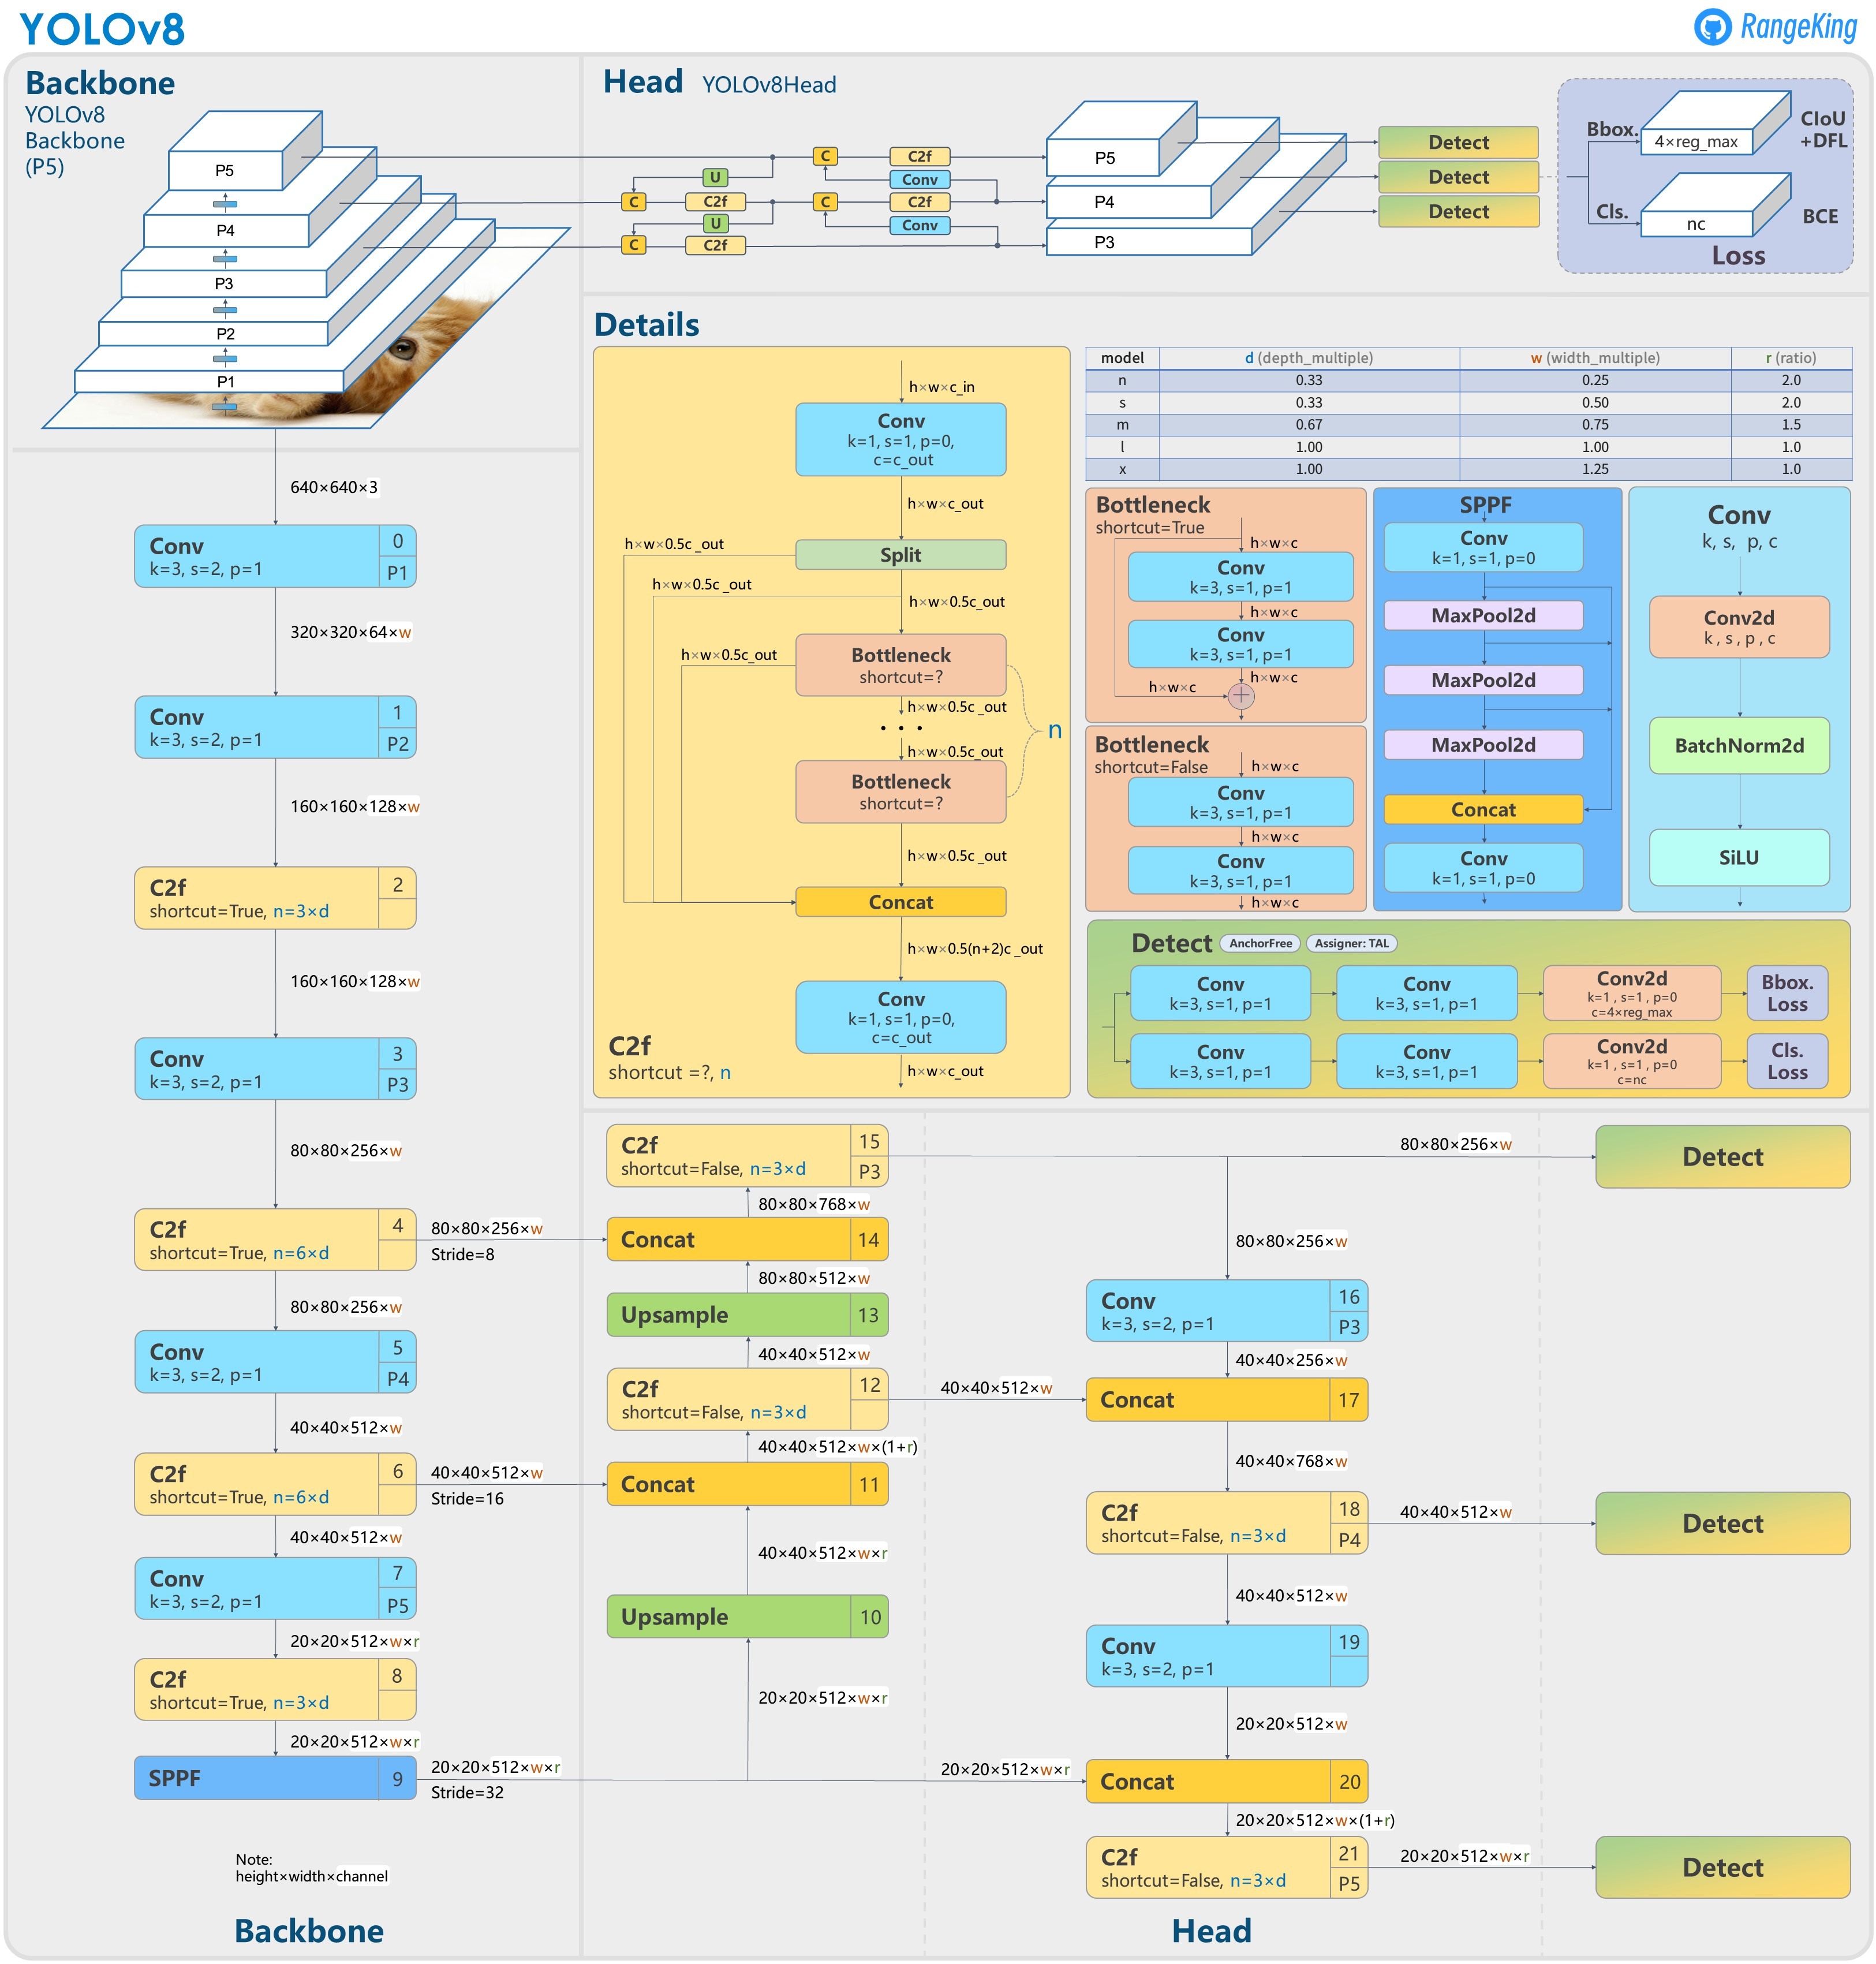
\includegraphics[width=\textwidth]{yolov8_model_architecture.jpg}
    \label{fig:yolov8-model-architecture}
\end{figure}
\clearpage
\hidsection{\acf{lvgl}}
This graphics library \autocite{LVGLLightVersatile} is a popular choice amongst embedded system engineers and has seen much usage, due to its portable support for a wide range of target architectures and devices. Its performance works well in resource constrained systems.\\
The library is generally very flexible, providing a rich set of widget types \autocite{WidgetsLVGLDocumentation} and layout systems (flex, grid), which allow developers to create complex and custom \ac{ui}. Fig.\ref{fig:lvgl-musicplayer-demo} and Fig.\ref{fig:lvgl-printer-demo} showcase some of the \ac{ui} capabilities of the library, with more available on their web page \autocite{llcLiveDemosTest}.\\
\begin{figure}
    \caption{\ac{lvgl} music player demo \autocite{llcLiveDemosTest}}
    \centering
    
\includegraphics[height=0.2\textheight]{lvgl-musicplayer-demo.png}
    \label{fig:lvgl-musicplayer-demo}
\end{figure}
\begin{figure}
    \caption{\ac{lvgl} printer demo \autocite{llcLiveDemosTest}}
    \centering
    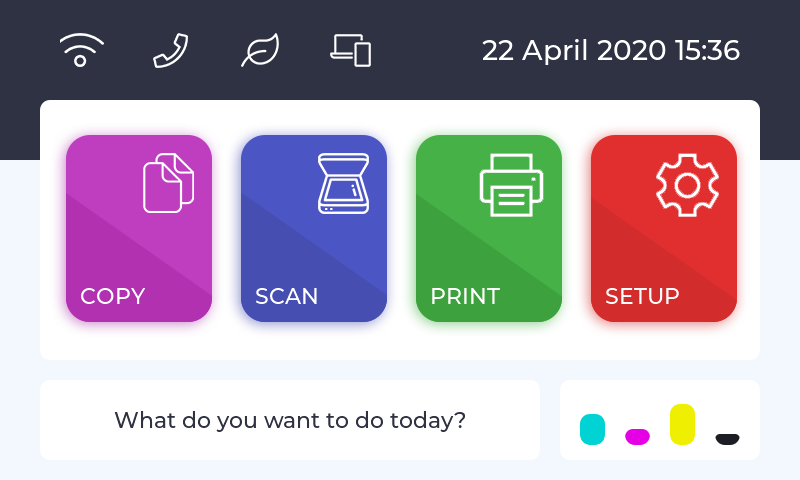
\includegraphics[height=0.2\textheight]{lvgl-printer-demo.png}
    \label{fig:lvgl-printer-demo}
\end{figure}
\clearpage
%%%%%%%%%%%%%%%%%%%%%%%%%%%%%%%%%%%%%%%% Start of generator development
\chapter{Development of synthesized datasets}
There generally is no available dataset for the target graphics library (\ac{lvgl}) of this research, so it was mandatory to create one during project development. Creating such a dataset artificially, meaning the images are not based on real world \acp{ui}, has the benefit of being able to adjust the size, variation and balance of the dataset very precisely. It would however be a complicated and time-consuming endeavour, if all of these \aclp{ui} would be created manually using regular \ac{lvgl} code, given that typical datasets for a \ac{ml} model of this type require hundreds of pictures or even more.\\
This is why a generator must be built, which is capable of creating and placing widgets in a structured manner. A screenshot of the displayed window needs to be captured and any metadata (size and position) of placed widgets must be gathered for creating corresponding annotations. The generator will also need to handle variation in visual representation of widgets, otherwise resulting datasets would be biased and detection accuracy of the model would be bad when used on screenshots of real-world examples, which typically incorporate varying visual representations of the same widget type.\\
In order to create variety in individual widgets, a randomized approach is used, where the outputted widgets will have varying styles applied to them. To gain more fine-control on the final visual representation of an created \ac{ui}, an additional design mode is necessary, where the creation of user interfaces can be statically described. The design mode will allow for creation of realistically looking \acp{ui}, while the random mode will allow for the creation of varying visual representation of the individual widgets.\\
Since the creation of a window in the generation process is singular, it will be necessary to have a mechanism to repeatedly call the generator to obtain a new image with each iteration. Using a modular approach, this paper will separate the generator, capable of producing a single image with annotations, from the so-called randomizer, which will loop the generator repeatedly for an arbitrary amount of iterations. This approach allows for a focused implementation that is capable of producing a good singular image, while having a secondary implementation that solely focuses on the organisation and creation of the dataset. Additionally, when written in the modular approach, it also allows for separation of concerns, where the generator will only need to deal with the intricacies of the \ac{lvgl} \ac{api}, while the randomizer can focus on the structural requirements of the dataset for the chosen model.\\
\section{First generator version in C}
The initial generator (v1) is forked from the existing VSCode simulator project of \ac{lvgl}.\autocite{LvglLv_port_pc_vscode2024} The simulator was stripped from any demo code and re-used as a binary with \ac{cli} arguments. For proper operation, the \code{lv\_conf.h} file was also modified, to increase allocation memory and deactivate unnecessary features. In the configuration, the default color depth was also modified to be 24 bit, so that output images would appear in higher quality. To be able to store screenshots, an additional library named \code{lv\_100ask\_screenshot} was used,\autocite{100askTeamLv_lib_100ask2024} which deals with the proper JPEG encoding using a \code{tiny\_jpeg} library internally.\\
Since the generator uses the allocation and storage mechanisms provided by \ac{lvgl}, it is necessary to use an identifier for the target storage system as prefix to the output filename. For this the \code{\textbackslash} character was chosen, so when supplying the \ac{cli} with a desired output filename, an example argument would look like this: \code{\textbackslash screenshot.jpg}\\
The following usage information will explain the available console arguments for this generator version:
\begin{listing}[htbp]
    \begin{minted}[
        frame=single,
        framesep=2mm,
        baselinestretch=1.2,
        bgcolor=white,
        fontsize=\footnotesize,
        breaklines
        ]{shell-session}
Usage: ./lvgl_ui_generator/build/bin/demo [OPTIONS]
Options:
-m <mode>                   Set the operation mode ("randomizer" or "design")
Randomizer Mode Options:
-w <width>                  Set the width of the UI
-h <height>                 Set the height of the UI
-c <widget_count>           Set the number of widgets to be randomized
-t <widget_types>           Comma-separated list of widget types to be used
-o <output_file>            Set the output file path
-d <delay_count>            Set the screenshot delay count
-l <layout>                 Set the layout type
    \end{minted}
    \caption{Usage instructions of LVGL generator v1}
\end{listing}
\\
When run, the generator will produce an image in the provided width and height, as shown in the example of Fig. \ref{fig:genv1example}\\
It will place randomly chosen widgets up to the given count on the window and use the selected layout (none, grid, flex) to structure them.\\
The layout structuring of widgets helped in outputting more placement variation in the final image. When using \code{flex}, the created widgets are aligned and will wrap onto the next line if they run out of width. In the \code{grid} layout, widgets would be placed in a grid-like pattern over the whole image. Finally in the \code{none} layout, widgets would be absolutely positioned randomly over the screen, sometimes also causing overlap of widget types.
\begin{figure}
    \caption{Example output of generator v1 (640x640, 40 random widgets, flex)}
    \centering
    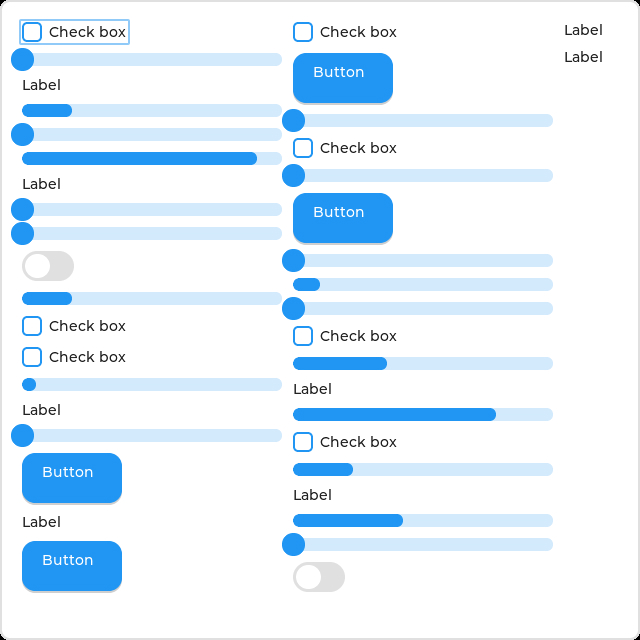
\includegraphics[width=\textwidth]{generator_v1_example.jpg}
    \label{fig:genv1example}
\end{figure}
\clearpage
\subsection{Development issues}
During development and testing of the first generator, it became apparent, that implementing further widget types would create a lot of complexity due to parameter passing in code. Since the C language does not inherently have classes, it was considered to be much more difficult to implement multiple widget types, each of which require a different set of options to be displayed properly.\\
Additionally, issues like segmentation faults due to window deletion occurred, which were inherited from the forked project. The implementation of a design mode was attempted, but this only increased complexity, which resulted in more unreliability of the program, despite the authors experience in the language. Frequent errors in compilation as well as a high compilation time due to the included \ac{lvgl} examples, which the author was not able to remove, were halting and slowing down development time. A lot of features \textit{(widget styles and states, widget property randomization, ...)} were still left to be implemented at a low level and C being a systems programming language, it was becoming too big of a problem for the project.\\\\
The general implementation based on C proved to be much more error-prone as a result of these issues and was therefor considered too complex for usage in a generation pipeline. A new solution was sought after, which would allow implementation of the generator in a more resilient and forgiving programming language.\\
\ac{lvgl} provides C bindings \autocite{LvglLv_binding_micropythonLVGL} for usage and implementation in other programming languages. A language promoted by the creators themselves is micropython \autocite{LvglLv_micropythonMicropython}, which is a reduced implementation of python for running on hardware. While the issues faced with the initial generator certainly are solvable, there existed no premise to continue in the C language. A new version in that language was considered to be a simpler approach that would refocus the project on the dataset creation matter at hand.
\clearpage
\section{Second generator version in Micropython}
The second generator version is implemented in micropython, and was started as a fresh project using the \code{lv\_micropython} project \autocite{LvglLv_binding_micropythonLVGL} as a necessary sub-module for compiling the micropython binary including the \code{lv\_bindings} module \autocite{LvglLv_micropythonMicropython}.\\
Rewriting the functionality of the initial generator was much simpler, as the binary comes with \code{argparse} for easily creating a \ac{cli} interface. Having the functionality of classes, it was also easier to differentiate between the two modes with their own source files. Widget creation was divided into separate functions, one for each widget type, and then called via a mapping of the type name to the creation function. This proved to be much more maintainable throughout project development and issues were able to be faced on an individual basis per implemented type.\\
Both modes provide a \code{get\_ui} function to retrieve the top-level container and all its children in a dictionary object format, containing all relevant metadata information gathered through usage of the \code{coords\_t} object. This \ac{lvgl} object is necessary, as it stores the coordinates of a widget in relation to the whole window, while other methods usually provide this information in relation to the parent container that the widget resides in.\\
The retrieved container is passed to a screenshot function, which uses a manually added JPEG encoding from the \code{flat} project \autocite{FlatFlatJpeg} to create an image. Using the coordinate metadata, the annotation file of the resulting image is created in \ac{yolo} format (\code{class center\_x center\_y center\_width center\_height}) and also normalized if the user provides the corresponding flag.
A resulting example image using design mode is illustrated in Fig.\ref{fig:genv2example} and its corresponding annotation file is listed below.\\
The following widget types were implemented and used in this generator version:
\begin{itemize}
  \begin{AutoMultiColItemize}
    \item Arc
    \item Bar
    \item Button
    \item Buttonmatrix
    \item Calendar
    \item Checkbox
    \item Dropdown
    \item Label
    \item Roller
    \item Scale
    \item Slider
    \item Spinbox
    \item Switch
    \item Table
    \item Textarea
  \end{AutoMultiColItemize}
\end{itemize}
% TODO arrange the figure and annotation to be alongside each other
\begin{figure}
    \caption{Example output of generator v2 (640x640, design, widget\_showcase.json)}
    \centering
    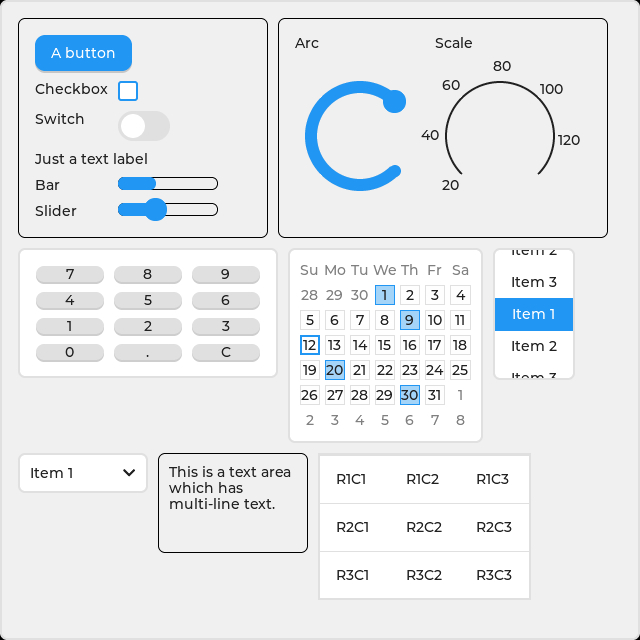
\includegraphics[height=0.4\textheight]{generator_v2_example.jpg}
    \label{fig:genv2example}
\end{figure}
\begin{listing}[htbp]
    \begin{minted}[
        frame=single,
        framesep=2mm,
        baselinestretch=1.2,
        bgcolor=white,
        fontsize=\footnotesize
        ]{shell-session}
textarea 0.3625 0.784375 0.234375 0.15625
table 0.6625 0.821875 0.3328125 0.2296875
checkbox 0.2046875 0.140625 0.04375 0.03125
arc 0.5609375 0.2109375 0.203125 0.203125
label 0.0734375 0.2875 0.0390625 0.025
label 0.0859375 0.328125 0.065625 0.025
label 0.478125 0.065625 0.0375 0.025
label 0.7078125 0.065625 0.059375 0.025
label 0.1109375 0.1375 0.1140625 0.025
bar 0.2609375 0.2859375 0.15625 0.0203125
label 0.0921875 0.184375 0.078125 0.025
label 0.1421875 0.246875 0.1765625 0.025
switch 0.2234375 0.1953125 0.08125 0.046875
buttonmatrix 0.2296875 0.4875 0.40625 0.203125
button 0.1296875 0.08125 0.1515625 0.05625
calendar 0.6015625 0.5390625 0.3046875 0.3046875
scale 0.7796875 0.2109375 0.203125 0.203125
slider 0.2609375 0.3265625 0.15625 0.0203125
roller 0.8328125 0.4890625 0.128125 0.20625
dropdown 0.128125 0.7375 0.203125 0.0625
    \end{minted}
    \caption{Generated annotation file for example output of generator v2}
\end{listing}
\clearpage
\hidsubsubsection{Distorted output images due to render race conditions}
The used snapshot \ac{api} sometimes causes output issues, since race-conditions can occur due to render updates while the referenced image data is still being encoded, resulting in distorted or sheared images as seen in the example Fig.\ref{fig:genv2distortedexample}. This largely originates from adding the JPEG encoding in micropython, which inherently is much slower than its C counterpart. While the issue was not solved during paper development due to its late discovery, a problem solution using a compiled C module of the latest libjpeg-turbo \autocite{LibjpegturboLibjpegturbo2024} version was discussed in development forums of \ac{lvgl} \autocite{HowCanStore2024}. Adding this module will improve encoding speed and thus not face race conditions due to underlying render updates by \ac{lvgl}. Images which had this issue needed to be regenerated and datasets were fixed manually.
\begin{figure}
    \caption{Example image with distortions from generator v2 (640x640)}
    \centering
    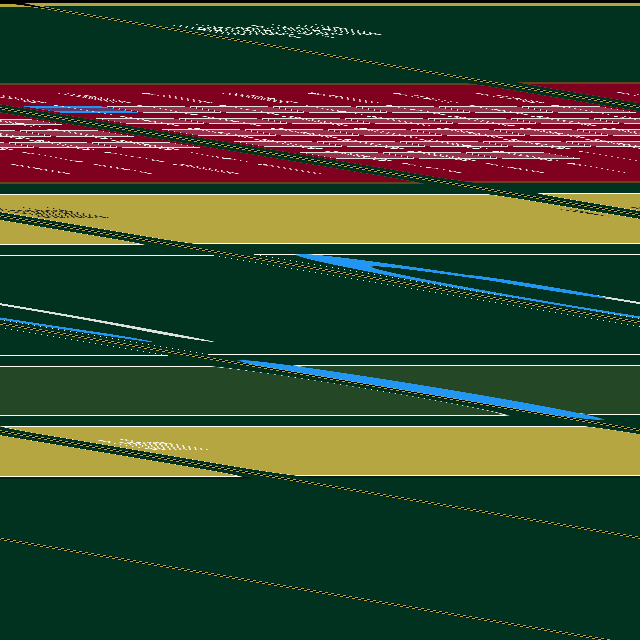
\includegraphics[height=0.4\textheight]{distorted_image_example.jpg}
    \label{fig:genv2distortedexample}
\end{figure}\\
\hidsubsubsection{Memory allocation errors}
Since the image encoding takes place in micropython, it actually takes up a lot more memory in heap. When creating and encoding images with the generator, it may result in memory allocation errors, depending on available memory on the running machine. This issue is not solved in the final generator version of the paper and was circumvented by retry mechanisms when creating image files using the dataset pipeline.
\newpage
\section{Random mode}
In random mode, the generator will produce a window of desired width and height. It randomly chooses widgets from the user provided type list and places them into a container. Since absolute positioning proved to be most suitable for random generation, the implementation of layouts was omitted. To avoid overlap, a spatial map was used, to find free space in the window during widget creation and placement.\\
The usage description in Listing \ref{code:genv2usage} provides an overview of the parameters for this mode.
\begin{listing}[htbp]
    \begin{minted}[
        frame=single,
        framesep=2mm,
        baselinestretch=1.2,
        bgcolor=white,
        fontsize=\footnotesize,
        breaklines
        ]{shell-session}
usage: src/main.py [-h] [-m, --mode mode] [-?, --usage] [-n, --normalize] [-o, --output_file output_file] [-W, --width width] [-H, --height height] [-c, --widget_count widget_count] [-t, --widget_types widget_types+] [-l, --layout layout] [--random-state]

Process CLI arguments for the UI generator.

optional args:
  -h, --help                        show this message and exit
  -m, --mode                        mode the mode to run the program in
  -?, --usage                       Print usage information for that mode.
  -n, --normalize                   normalize the bounding boxes
  -o, --output_file output_file     The output file (screenshot)
  -W, --width width                 the width of the UI
  -H, --height height               the height of the UI
  -c, --widget_count widget_count   the count of widgets
  -t, --widget_types widget_types+  A list of widget types
  -l, --layout layout               the layout option
  --random-state                    Use a random state for each created widget (experimental)
    \end{minted}
    \caption{Usage instructions of LVGL generator v2 in random mode}
    \label{code:genv2usage}
\end{listing}
\subsection{Style and state variation}
When using random mode, the generator will randomize applied style of widgets to artificially create variation in created datasets. Additionally, there is an experimental feature, which will also randomize the state of widgets. The latter is not recommended for usage in training, as sometimes this might cause widgets to not be displayed if their state is invalid or disabled, which will confuse the model, as the created metadata will still include the annotation of said widget.\\
Listing \ref{code:randomized-properties} shows the properties and their range of possible values to be randomized. Listing \ref{code:randomized-state} shows the available states.
\begin{listing}[htbp]
    \begin{minted}[
        frame=single,
        framesep=2mm,
        baselinestretch=1.2,
        bgcolor=white,
        fontsize=\footnotesize,
        breaklines
        ]{python}
# List of style properties to randomize
properties = [
    ('set_bg_color', lv.color_make),
    ('set_bg_opa', lambda: random.randint(0, 100)),
    ('set_border_color', lv.color_make),
    ('set_border_opa', lambda: random.randint(0, 100)),
    ('set_border_width', lambda: random.randint(0, 10)),
    ('set_outline_width', lambda: random.randint(0, 10)),
    ('set_outline_color', lv.color_make),
    ('set_outline_opa', lambda: random.randint(0, 100)),
    ('set_shadow_width', lambda: random.randint(0, 15)),
    ('set_shadow_offset_x', lambda: random.randint(0, 10)),
    ('set_shadow_offset_y', lambda: random.randint(0, 10)),
    ('set_shadow_color', lv.color_make),
    ('set_shadow_opa', lambda: random.randint(0, 100)),
    ('set_line_width', lambda: random.randint(0, 10)),
    ('set_line_dash_width', lambda: random.randint(0, 10)),
    ('set_line_dash_gap', lambda: random.randint(0, 10)),
    ('set_line_rounded', lambda: random.choice([True, False])),
    ('set_line_color', lv.color_make),
    ('set_line_opa', lambda: random.randint(0, 100)),
    ('set_text_color', lv.color_make),
    ('set_text_opa', lambda: random.randint(0, 100)),
    ('set_text_letter_space', lambda: random.randint(0, 10)),
    ('set_text_line_space', lambda: random.randint(0, 10)),
    ('set_opa', lambda: random.randint(0, 100)),
    ('set_align', lambda: random.choice([lv.ALIGN.CENTER, lv.ALIGN.TOP_LEFT, lv.ALIGN.TOP_RIGHT, lv.ALIGN.TOP_MID, lv.ALIGN.BOTTOM_LEFT, lv.ALIGN.BOTTOM_RIGHT, lv.ALIGN.BOTTOM_MID, lv.ALIGN.LEFT_MID, lv.ALIGN.RIGHT_MID, lv.ALIGN.DEFAULT])),
    ('set_pad_all', lambda: random.randint(0, 10)),
    ('set_pad_hor', lambda: random.randint(0, 10)),
    ('set_pad_ver', lambda: random.randint(0, 10)),
    ('set_pad_gap', lambda: random.randint(0, 10)),
    ('set_pad_top', lambda: random.randint(0, 10)),
    ('set_pad_bottom', lambda: random.randint(0, 10)),
    ('set_pad_left', lambda: random.randint(0, 10)),
    ('set_pad_right', lambda: random.randint(0, 10)),
    ('set_pad_row', lambda: random.randint(0, 10)),
    ('set_pad_column', lambda: random.randint(0, 10)),
    ('set_margin_top', lambda: random.randint(0, 10)),
    ('set_margin_bottom', lambda: random.randint(0, 10)),
    ('set_margin_left', lambda: random.randint(0, 10)),
    ('set_margin_right', lambda: random.randint(0, 10))
]
    \end{minted}
    \caption{Available style properties which are randomized in given value range}
    \label{code:randomized-properties}
\end{listing}
\begin{listing}[htbp]
    \begin{minted}[
        frame=single,
        framesep=2mm,
        baselinestretch=1.2,
        bgcolor=white,
        fontsize=\footnotesize,
        breaklines
        ]{python}
def randomize_state(widget: lv.obj):
    if hasattr(widget, "set_state"):
        state = random.choice([lv.STATE.CHECKED, lv.STATE.DISABLED, lv.STATE.FOCUSED, lv.STATE.PRESSED, lv.STATE.HOVERED, lv.STATE.EDITED])
        widget.set_state(state, True) # Add the state
    else:
        raise AttributeError(f"Widget {widget} does not have a 'state' property.")
    \end{minted}
    \caption{Available state properties which are randomized in given options}
    \label{code:randomized-state}
\end{listing}
\clearpage
\section{Design mode}
In design mode, the generator will parse a provided \ac{json} file and create a \ac{ui} according to the specified design. This mode allows for creation of a static \ac{ui} design, which more resembles the expectation of a realistic interface in comparison to the random mode. To allow for variation in this mode, a special type \code{random} is available, which randomly chooses widgets from a given type list and randomizes their appearance. This option is similar to random mode and allows for randomization in specific portions of the \ac{ui}, while keeping the rest statically defined. In the design file, various styles can be defined. Multiple styles can then be applied to individual widgets and containers by name reference. In general, all possible \textit{setter} properties of \ac{lvgl} styles are allowed, as the implementation checks for the availability of the corresponding setter attribute on a \code{lv.style\_t} object.\\
Since the design mode only requires a single parameter \textit{(i.e. the path to the design file)}, no further usage instructions are provided in this paper.
\hidsubsection{Design file rules}
The creation of design files require a certain set of rules that need to be followed, in order for the creation to work properly.
\begin{enumerate}
    \item It is mandatory that the first widget object in \code{root} is a container, as the root widget is always a container.
    \item The title of the window is not mandatory and not used by the generator. It is only there for reference to the user for describing and recognizing the contents of a design file.
    \item The \code{styles} object is optional and can be omitted if no styles are defined.
    \item Added styles are referenced by their name in the \code{style} array of each widget. If a style is not found, the generator will throw a \code{ValueError}.
    \item A style defines a list of properties that are applied to widgets via the usage of a \code{lv.style\_t} object. The possible properties are the same as documented in the \ac{lvgl} \ac{api} for styles \autocite{Lv_style_genLVGLDocumentation}.
Properties are verified by checking if the specified name has a corresponding \code{setter} attribute in the object. This is done by appending \code{set\_} to the property name, thus the user is required to use the property setter function names without the prefix. For example, to set the background color of a widget, one would use the property \code{bg\_color}. The generator will then look for the \code{set\_bg\_color} attribute in the object and apply the converted value to it.
    \item If a provided property inside a style object does not actually correspond to an available attribute, the generator will ignore it and continue.
    \item Values supplied to style properties are converted according to the required type of the property. Some properties taking in special objects, like colors, require a specific string to be supplied (e.g. \code{\#RRGGBB} for any color property or \code{top-left} for the align property).
    \item If value conversion fails, the property is ignored and the generator will ignore it and continue.
    \item The id property is mandatory for widgets of type container, as it is required to reference the container inside the children array, when the special widget type random is used.
    \item The special widget type random may be used to supply a list of widget types for the generator to randomly choose from and then create a random widget in similar fashion to the random mode. This is useful for randomizing widgets in certain areas of the UI, while keeping the rest of the UI static.
\end{enumerate}
\newpage
\subsection{JSON schema}
In order to validate design files before providing them to the generator, a regular python script is used. This was not included in the generator, as the corresponding package is not available in micropython. The schema was purposely made more strict than what the generator requires, so that validation errors could be provided to the later used \ac{llm}, to offer more detailed guidance during design generation.
Listing \ref{code:validate-design-script} shows a simple example script to validate a design file with the available schema \autocite{UidetectorSchemaDesign_file} in the source repository.
\begin{listing}[htbp]
    \begin{minted}[
        frame=single,
        framesep=2mm,
        baselinestretch=1.2,
        bgcolor=white,
        fontsize=\footnotesize,
        breaklines
        ]{python}
def load_json_file(filepath: str):
    import json
    with open(filepath, 'r') as f:
        return json.load(f)

def verify_design_from_file(design_file: str, schema_file: str) -> tuple[bool, Exception]:
    from jsonschema import validate
    from jsonschema.exceptions import ValidationError
    design = load_json_file(design_file)
    schema = load_json_file(schema_file)
    try:
        validate(instance=design, schema=schema)
        print(f"Provided design file {design_file} is valid.")
        return True, None
    except ValidationError as e:
        print(f"Provided design file {design_file} is invalid:\n{e}")
        return False, e

if __name__ == '__main__':
    verify_design_from_file('path/to/design_file.json', 'path/to/design_file.schema.json')
    \end{minted}
    \caption{Exemplary validation code for design file using JSON schema}
    \label{code:validate-design-script}
\end{listing}
\clearpage
\section{Dataset creation}
Both generator modes only ever produce a single image output with a corresponding text file in the \ac{yolo} annotation format. This choice was intended to allow for a separate implementation which will handle the organization of created files, by repeatedly calling the generator and moving the outputs into a dataset folder structure. It was also a necessary choice, as the micropython programming language would have been very limiting for implementing third-party integration.\\
Furthermore, it also allowed for balancing the representation of classes in random mode, by removing a type from the provided widget list, once a certain threshold of instances for that class is reached.\\
The dataset creation concept is further illustrated in Fig.\ref{fig:dataset-creation-random} and Fig.\ref{fig:dataset-creation-design}.\\
The produced annotations in each iteration are post-processed before they are moved into the dataset structure. Widgets that are placed out-of-bounds of the window have annotation values which are not usable for model training, as such they will be removed from the annotation file during this step. The label modifications are generally minor, since they occur rarely, and their affect on model performance is negligible. In the annotations, the written class names also need to be processed, since the \ac{yolo} model cannot interpret classes from their string representation, so they are replaced by their index in the list of implemented types.
\begin{figure}[!htbp]
    \caption{Dataset creation concept using random mode}
    \centering
    \includesvg[width=\textwidth,keepaspectratio]{PICs/Framework-Generic_generator-random}
    \label{fig:dataset-creation-random}
\end{figure}
\begin{figure}[!htbp]
    \caption{Dataset creation concept using design mode with gpt}
    \centering
    \includesvg[width=\textwidth,keepaspectratio]{PICs/Framework-Generic_design-mode-gpt}
    \label{fig:dataset-creation-design}
\end{figure}
\clearpage
\subsection{Design contexts and themes}
Since creation of a large design dataset would additionally require the labor-intensive manual definition of a large set of designs, it was decided to use a \ac{llm} which would handle the creation of those design files. For that purpose, a list of 100x contexts and 100x themes was created. By unique pair combination, this creates a possible list of 10000 design contexts and themes to be provided to the \ac{llm}.\\
As illustrated in Fig.\ref{fig:dataset-creation-design}, the \ac{llm} would first be instructed to write out a design idea in the provided \ac{ui} context and style theme. Via a system prompt, the model is instructed to include the widgets to be used in the design, a high-level description of the \ac{ui} purpose and a structural description of what the \ac{ui} shall look like.\\
The idea output is then again fed into the \ac{llm} in a separate context and instructed to output a valid \ac{json} file. It additionally receives the \ac{json} schema as guidance on how to structure and construct the output \ac{json}. The resulting output of the model is then validated against the schema and any validation errors are fed back to the \ac{llm} for correction. Once an output design is valid, it will be stored and added to a design file list, to be generated in a following step. This loop can be repeated for a desired amount of design files, for up to 10000 generations, given our combination list of contexts and themes.
\subsection{Third-party integration} % ClearML & LLM (ChatGPT)
The dataset creation process relies heavily on third-party integration. To track individual versions of datasets, a popular experiment tracker named ClearML was used. In order to automate the design file creation process, the proprietary \ac{llm} named ChatGPT was used via OpenAIs available python package and \ac{api}.
\hidsubsubsection{Integration with ClearML}
Whenever a dataset creation starts, a new ClearML task is created and used for generating statistics about the process. The task stores all of the following information:
\begin{itemize}
    \item Console output of the script
    \item Scalar plots displaying generation statistics over iterations
    \item Metadata about dataset (file split of train,val,train)
    \item Artifacts (ZIP folder of dataset contents)
    \item Parameters of the script/task
    \item Machine environment information
    \item Version control information (diff, commit hash, ...)
\end{itemize}
All of that surrounding information regarding the creation process helps in getting a better understanding about errors and quality of the created dataset.
\hidsubsubsection{Integration with LLM (gpt-4-turbo)}
In order to generate design files at a larger scope, OpenAIs gpt-4-turbo model was used in the dataset creation process when using the design mode of generator v2. In order for the model to properly behave and generate usable output, the \ac{gpt} was instructed via system prompts.
The prompt was designed, so that the format of the idea is structurally similar through each iteration and proper output from the \ac{json} generation step can be expected. The used system prompt for the design \ac{json} can be seen in Listing \ref{code:gpt4-design-json-system-prompt}. Due to their length, the system prompt for the design idea and corresponding examples are omitted from the paper, but can be viewed in the source code repository \autocite{UidetectorSrcGenerate}.
\begin{listing}[htbp]
    \begin{minted}[
        frame=single,
        framesep=2mm,
        baselinestretch=1.2,
        bgcolor=white,
        fontsize=\footnotesize,
        breaklines
        ]{text}
You are a UI generator.
Your goal is to create a new single window UI using a specialized JSON format.
The format specification is available in the design.schema.json file below.
Follow the provided design guideline of the user when replicating the design idea using the structure of the JSON format.
Always output a valid JSON object that represents the UI design.

You ALSO MUST adhere to the following SPECIAL RULES:
- Never use 'grid' container. Use either 'none' or 'flex' container.
- Containers must be used to set style for the whole window or the specific group of widgets (such as background color and other general styles).
- Each widget placed inside a 'none' container must have an associated style defining its X and Y coordinates.
- Widgets may have multiple styles applied to them
- Window size MUST be 640 x 640 pixels
- You MUST make sure that coordinates of widgets do not overlap due to width and height of the widgets
- You MUST make sure that the widgets are within the window bounds (0, 0, 640, 640)
    \end{minted}
    \caption{System prompt for gpt-4-turbo generating design file (\ac{json})}
    \label{code:gpt4-design-json-system-prompt}
\end{listing}
\hidsubsection{Randomizer script}
In order to provide a randomizer script which does not rely on third-party integration, an extra module was created. The repository \autocite{HackXItUi_randomizer14d441c38a37850f4809471124bea3c36b9bc0b7} contains scripts for calling both generator versions. These scripts also repeatedly call the generator and allow for manual dataset creation, without necessity of additional third-party services. An optional mechanism to upload the created dataset to ClearML afterwards, if desired by the user, is implemented in v2.
\newpage
%%%%%%%%%%%%%%%%%%%%%%%%%%%%%%%%%%%%%%%% Start of model training
\chapter{Training of YOLO model}
The training process illustrated in Fig.\ref{fig:yolo-train} uses the already built training mechanisms of ultralytics \autocite{jocherUltralyticsYOLO2023} \ac{yolo} model version 8.1 \autocite{UltralyticsUltralyticsV8}. All experiments of the paper were performed using this model version and the specific python package version used was 8.1.47.
\begin{figure}[!htbp]
    \caption{YOLOv8 model training process}
    \centering
    \includesvg[width=\textwidth,keepaspectratio]{PICs/Framework-Generic_model-train}
    \label{fig:yolo-train}
\end{figure}
\section{Training tasks in ClearML}
Every training process of a \ac{yolo} model is automatically tracked via the existing integration of ClearML in the ultralytics \ac{yolo} engine. This was a crucial step in the creation of reproducible results, since all hyper-parameters of the training process are stored and the used dataset is referenced by a unique ID. This also allows for later modification of a training process, by cloning of the training task and manual editing of parameters in the cloned task.
\subsection{Training agents on local and remote machines}
In order to train models remotely on a more powerful machine than the authors laptop, a ClearML agent was setup using Google Colab. The creators of ClearML provide a simple mechanism and already defined notebook \autocite{ClearMLAgentGoogle} for starting such an agent. By having this agent readily available, any local or previously started training tasks could be remotely executed. The built integration uses docker containers to execute individual tasks and execution was therefor immutable once finalized. Such an agent was also started on the local machine of the author, to compare results between the two machines and for debugging purposes of the pipeline itself.
\section{Tuning for best hyperparameters}
In order to optimize the training process for a given dataset to determine the best set of hyper-parameters, the existing tuning process from the ultralytics engine \autocite{ultralyticsTuner} is used. This tuning process has automatic optimization features, choosing different optimizer algorithms for different epochs.
\section{Hyperparameter optimization}
The tune process by ultralytics was not always best for producing results. In some cases, the process failed to record the output model weights, despite reporting good results, which led to the creation of a custom \ac{hpo} pipeline.\\
ClearML offers mechanisms for performing \ac{hpo} \autocite{HyperparameterOptimizationClearML} on previously executed training tasks. For the optimization of parameters, the Optuna optimizer \autocite{OptunaHyperparameterOptimization} is used, which offers an algorithm to optimize for a given metric using either discrete value ranges or a defined set of scalar values. The open-source optimizer implementation would then determine the best hyper-parameters for the training task by running it multiple times with a different set of parameters determined by the algorithm, while tracking the target performance metrics. In all \ac{hpo} processes performed, the configured target metric was the \ac{map}, which shows the model performance across different levels of detection difficulty. The \ac{yolo} training process provides two \ac{map} metrics:
\begin{itemize}
    \item \ac{map}50 - Mean Average Precision at 50\% \ac{iou} threshold
    \item \ac{map}50-95 - Mean Average Precision averaged over \ac{iou} thresholds from 50\% to 95\% (at 5\% steps)
\end{itemize}
The author chose the \ac{map}50-95 metric, as it provided a more comprehensive view of the models performance, which was representative of an overall better accuracy and recall.
\section{Note on ClearML pipelines}
The author calls the implementations in the UI detector repository pipelines, even though they are simply python scripts with a \ac{cli}. They are however implemented in the recommended pattern \autocite{PipelineDecoratorClearML} that would later allow these individual scripts to be adapted to pipelines. This is also the reason that all imports that a function requires are located in the corresponding function body and not the top of the script. Pipelines were however not used during paper development, as they require a bit more implementation to work properly and it was considered out-of-scope for this paper to do so.
\clearpage
%%%%%%%%%%%%%%%%%%%%%%%%%%%%%%%%%%%%%%%% Start of results
\chapter{Research results}
The final project resulted in the creation of a custom dataset generator capable of producing \ac{ui} screenshot images with corresponding widget annotations. It provides two modes of operation, which can be used to create datasets of varying image sizes, styling properties and used widget types.
In addition to that, a \ac{json} design parser was written, which converts a design specification written in accordance to a \ac{json} schema into an image representing a realistically looking \ac{ui}. Multiple pipelines with integration to ClearML were written, to aid in dataset generation, \ac{yolo} model training and \acf{hpo}.
\section{Model performance}
The created generators were used in the research to train a baseline model based on a random dataset. The performance of this baseline model showed such good results, that the author doubted the viability in real-world scenarios, since the resulting metric scores showcased a form of over-optimization for the case of detecting widget types on a white background.\\
In response to that, another dataset using the implemented design mode was created with the help of an \ac{llm} to produce the necessary design files. The main purpose of the design mode is to create more realistic looking \acp{ui}, with an overall theme applied in the form of styles, which got rid of the white background and allowed the widgets to blend in more within the window.\\
The improved model was trained on the generated design dataset and shows a decrease in performance when compared to the baseline model. The drop in performance is attributed to the increased difficulty for the model when detecting widgets on colored and styled backgrounds, which slightly blends the visible features of individual widgets with their surroundings, making them harder to detect.\\
\begin{table}[]
    \centering
    \begin{tabular}{c|c|c|c|c}
         Dataset & mAP50 & mAP50-95 & fitness & model\_variant \\
         Train (random) & 0.95312 & 0.86023 & 0.86952 & yolov8n \\
         Train (design) & 0.77673 & 0.74507 & 0.74824 & yolov8n
    \end{tabular}
    \caption{Training results with random \& design dataset}
    \label{tab:overall-training-results}
\end{table}\\
Visualizations of training results for the random dataset are depicted in Fig.\ref{fig:random-training-results},\ref{fig:random-training-confusion},\ref{fig:random-training-labels} and \ref{fig:random-training-f1}.\\
\begin{figure}
    \caption{Random dataset training - results}
    \centering
    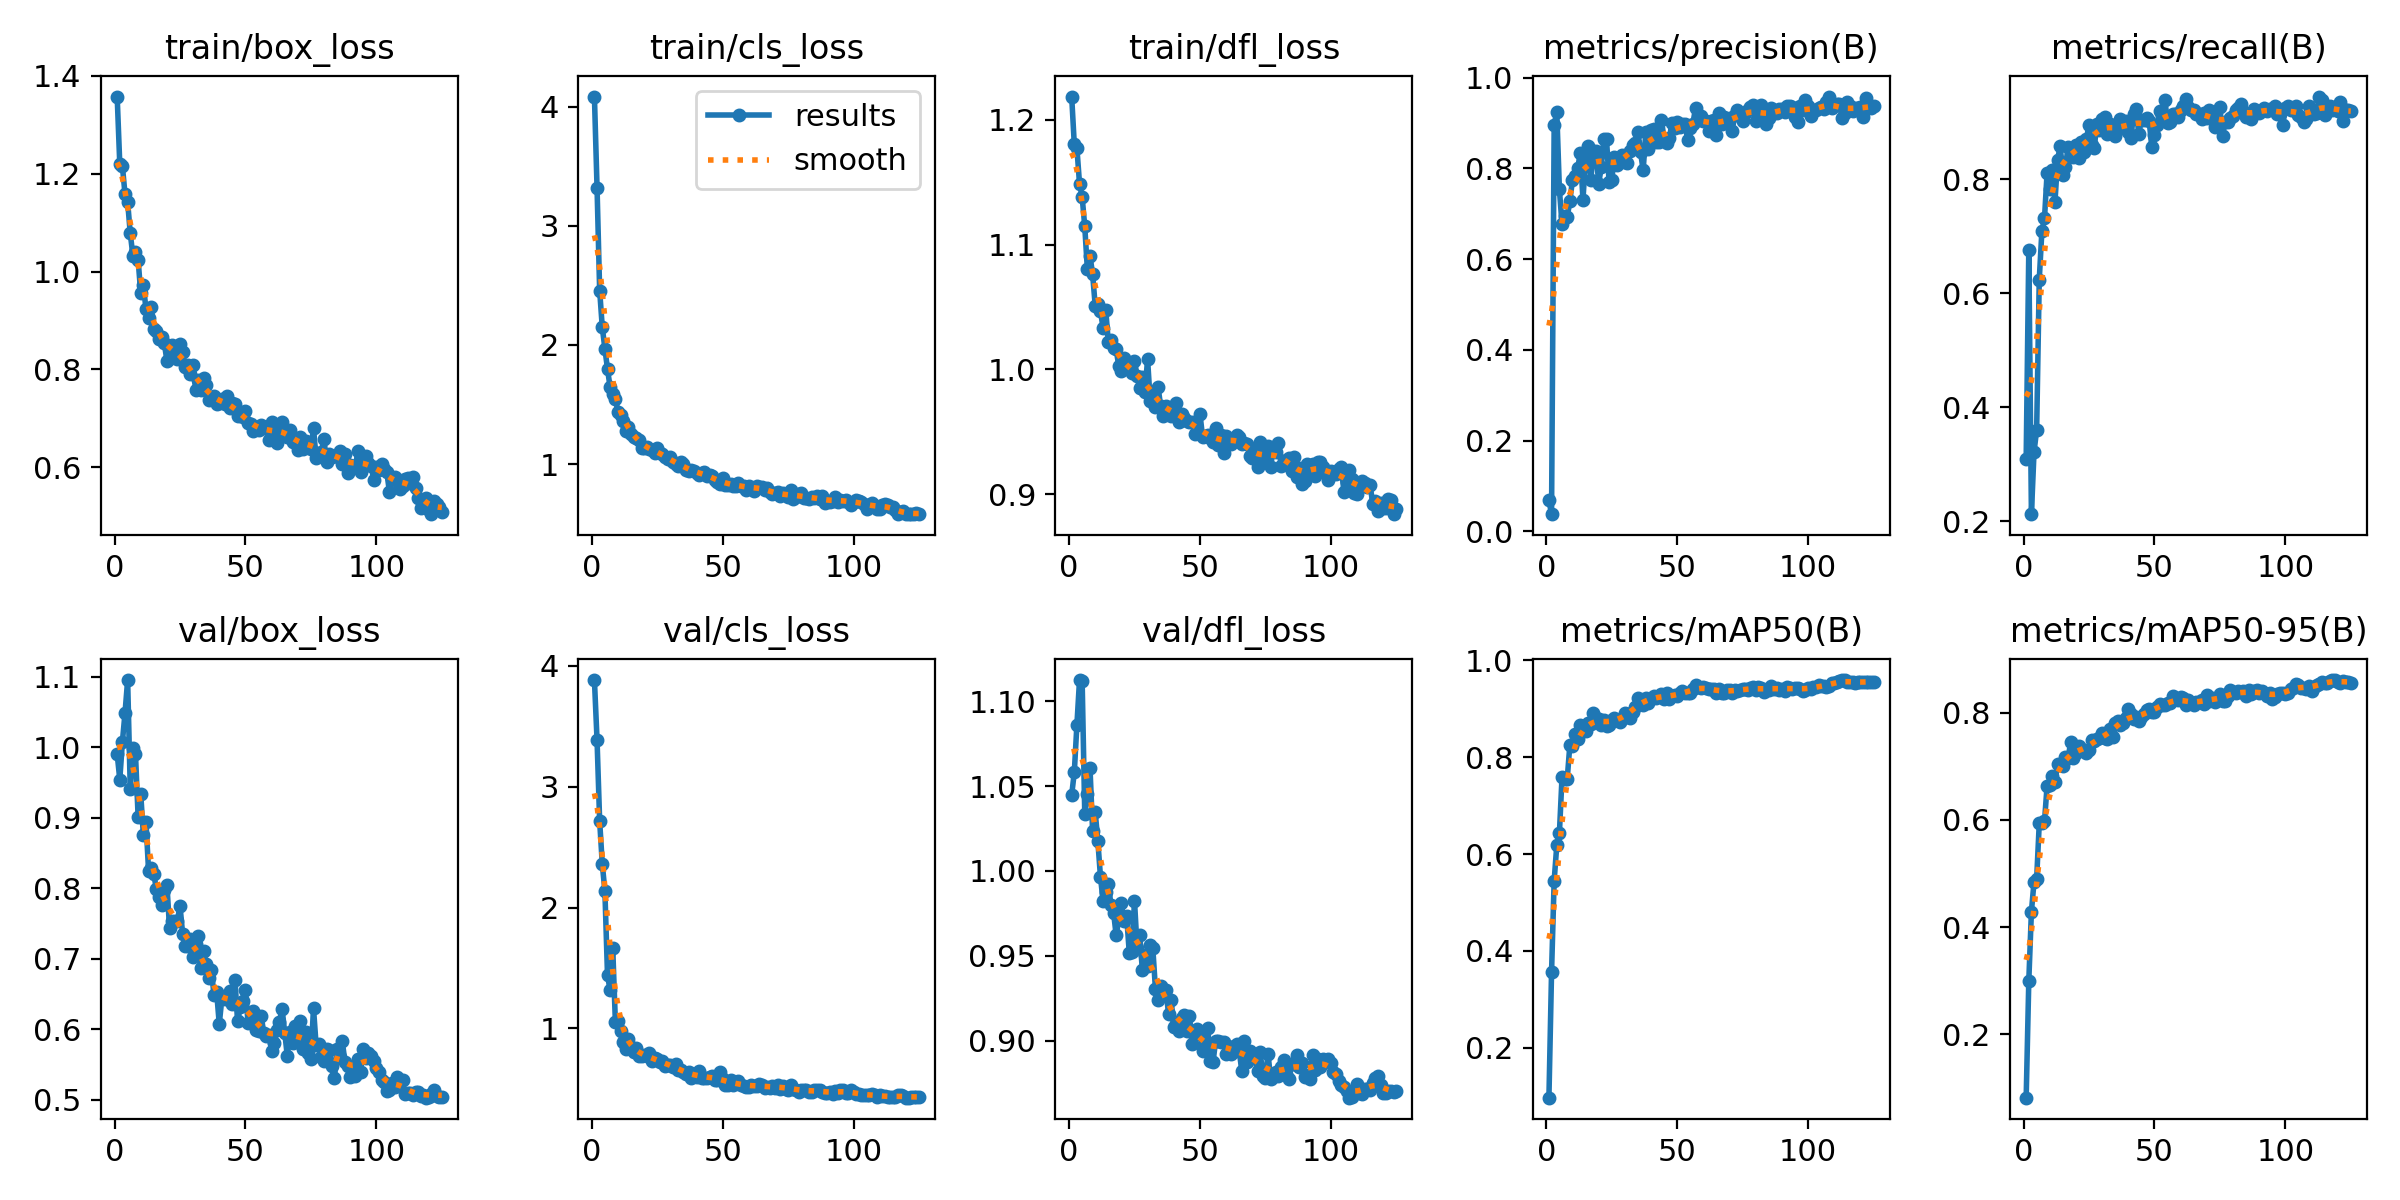
\includegraphics[width=\textwidth]{PICs/train371/results.png}
    \label{fig:random-training-results}
\end{figure}
\begin{figure}
    \caption{Random dataset training - confusion matrix (normalized)}
    \centering
    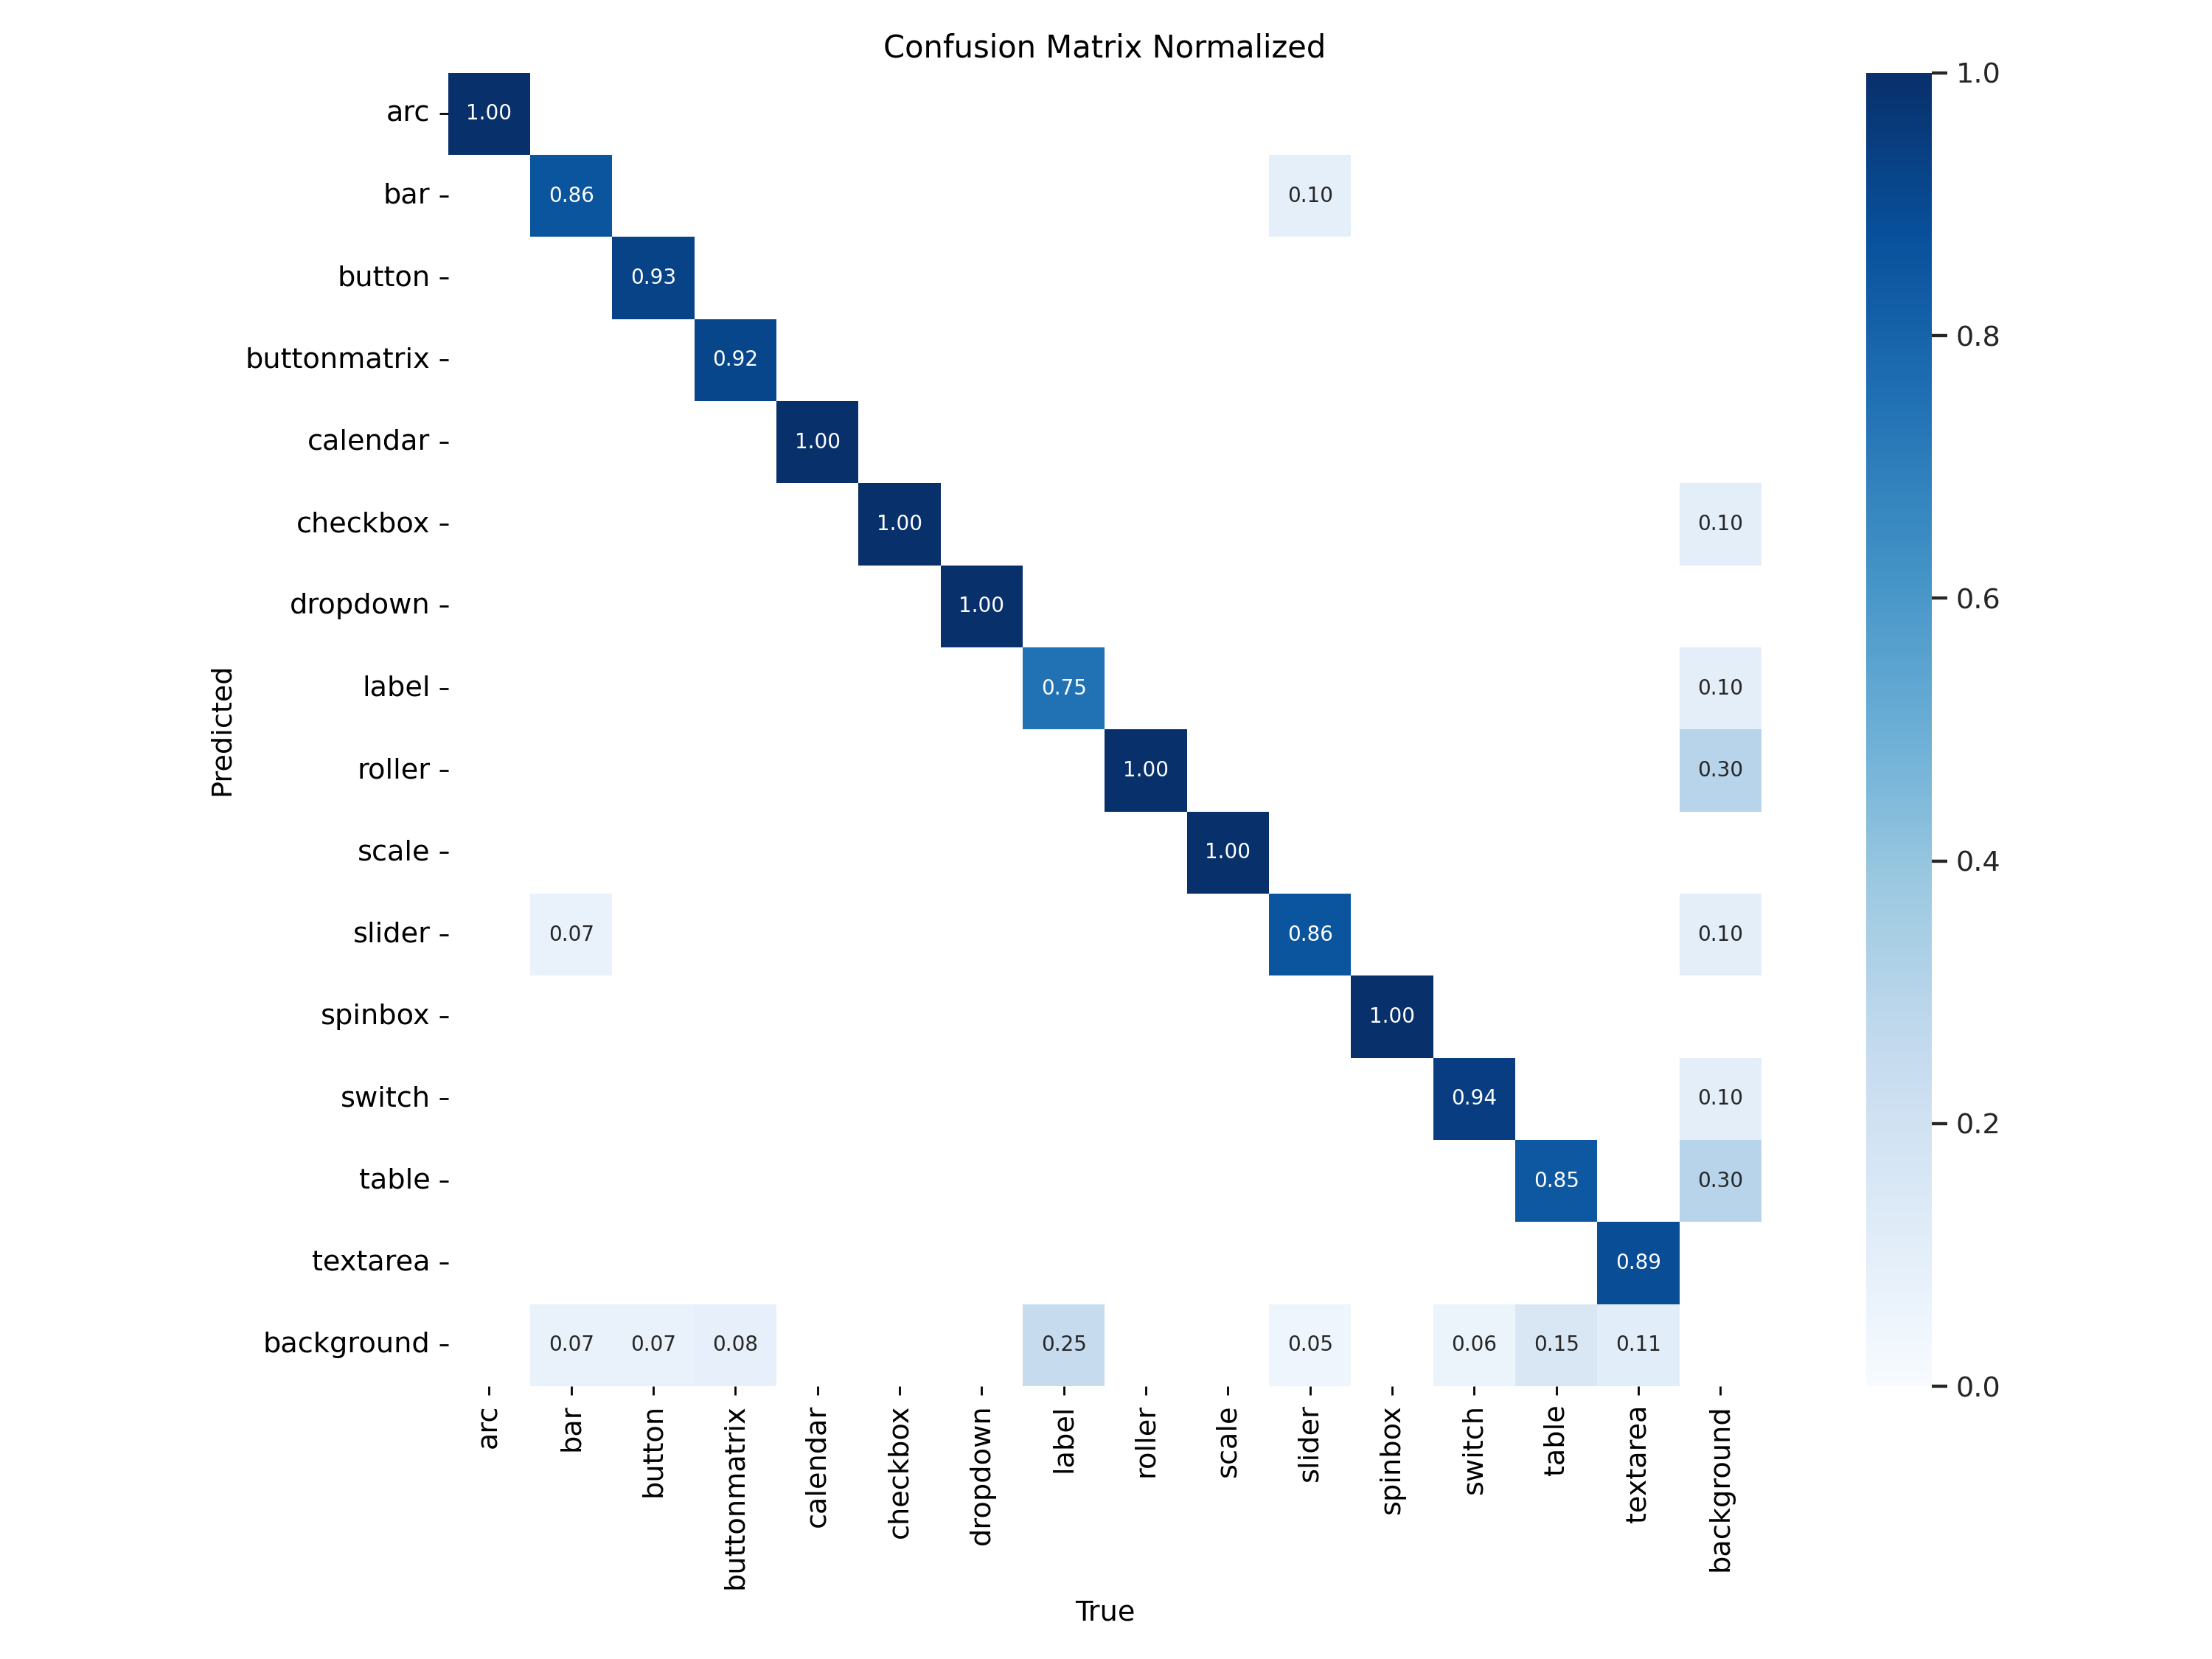
\includegraphics[width=\textwidth]{PICs/train371/confusion_matrix_normalized.png}
    \label{fig:random-training-confusion}
\end{figure}
\begin{figure}
    \caption{Random dataset training - label distribution}
    \centering
    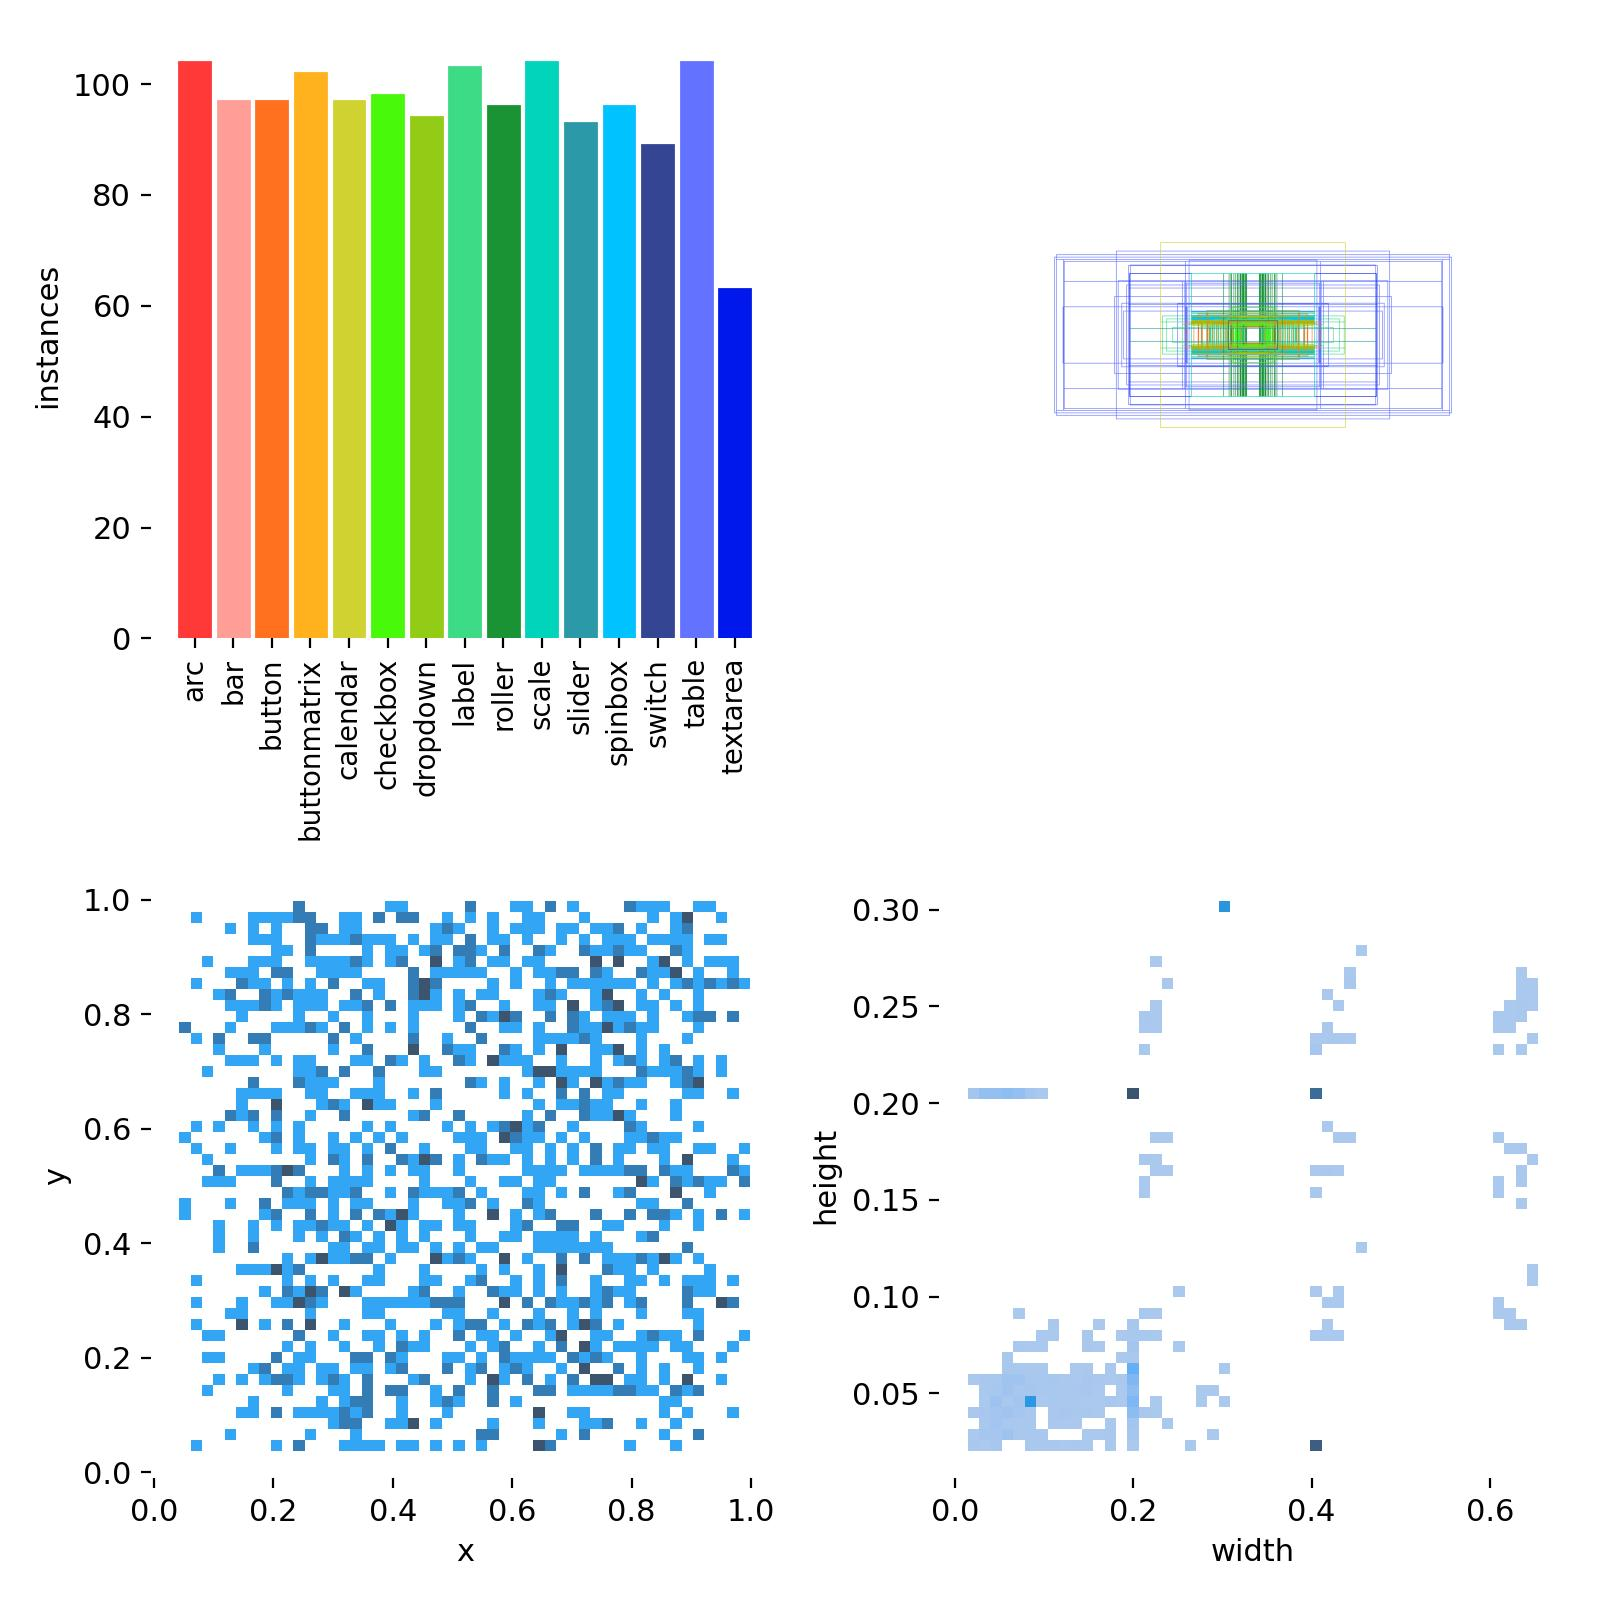
\includegraphics[width=\textwidth]{PICs/train371/labels.jpg}
    \label{fig:random-training-labels}
\end{figure}
\begin{figure}
    \caption{Random dataset training - F1 curve}
    \centering
    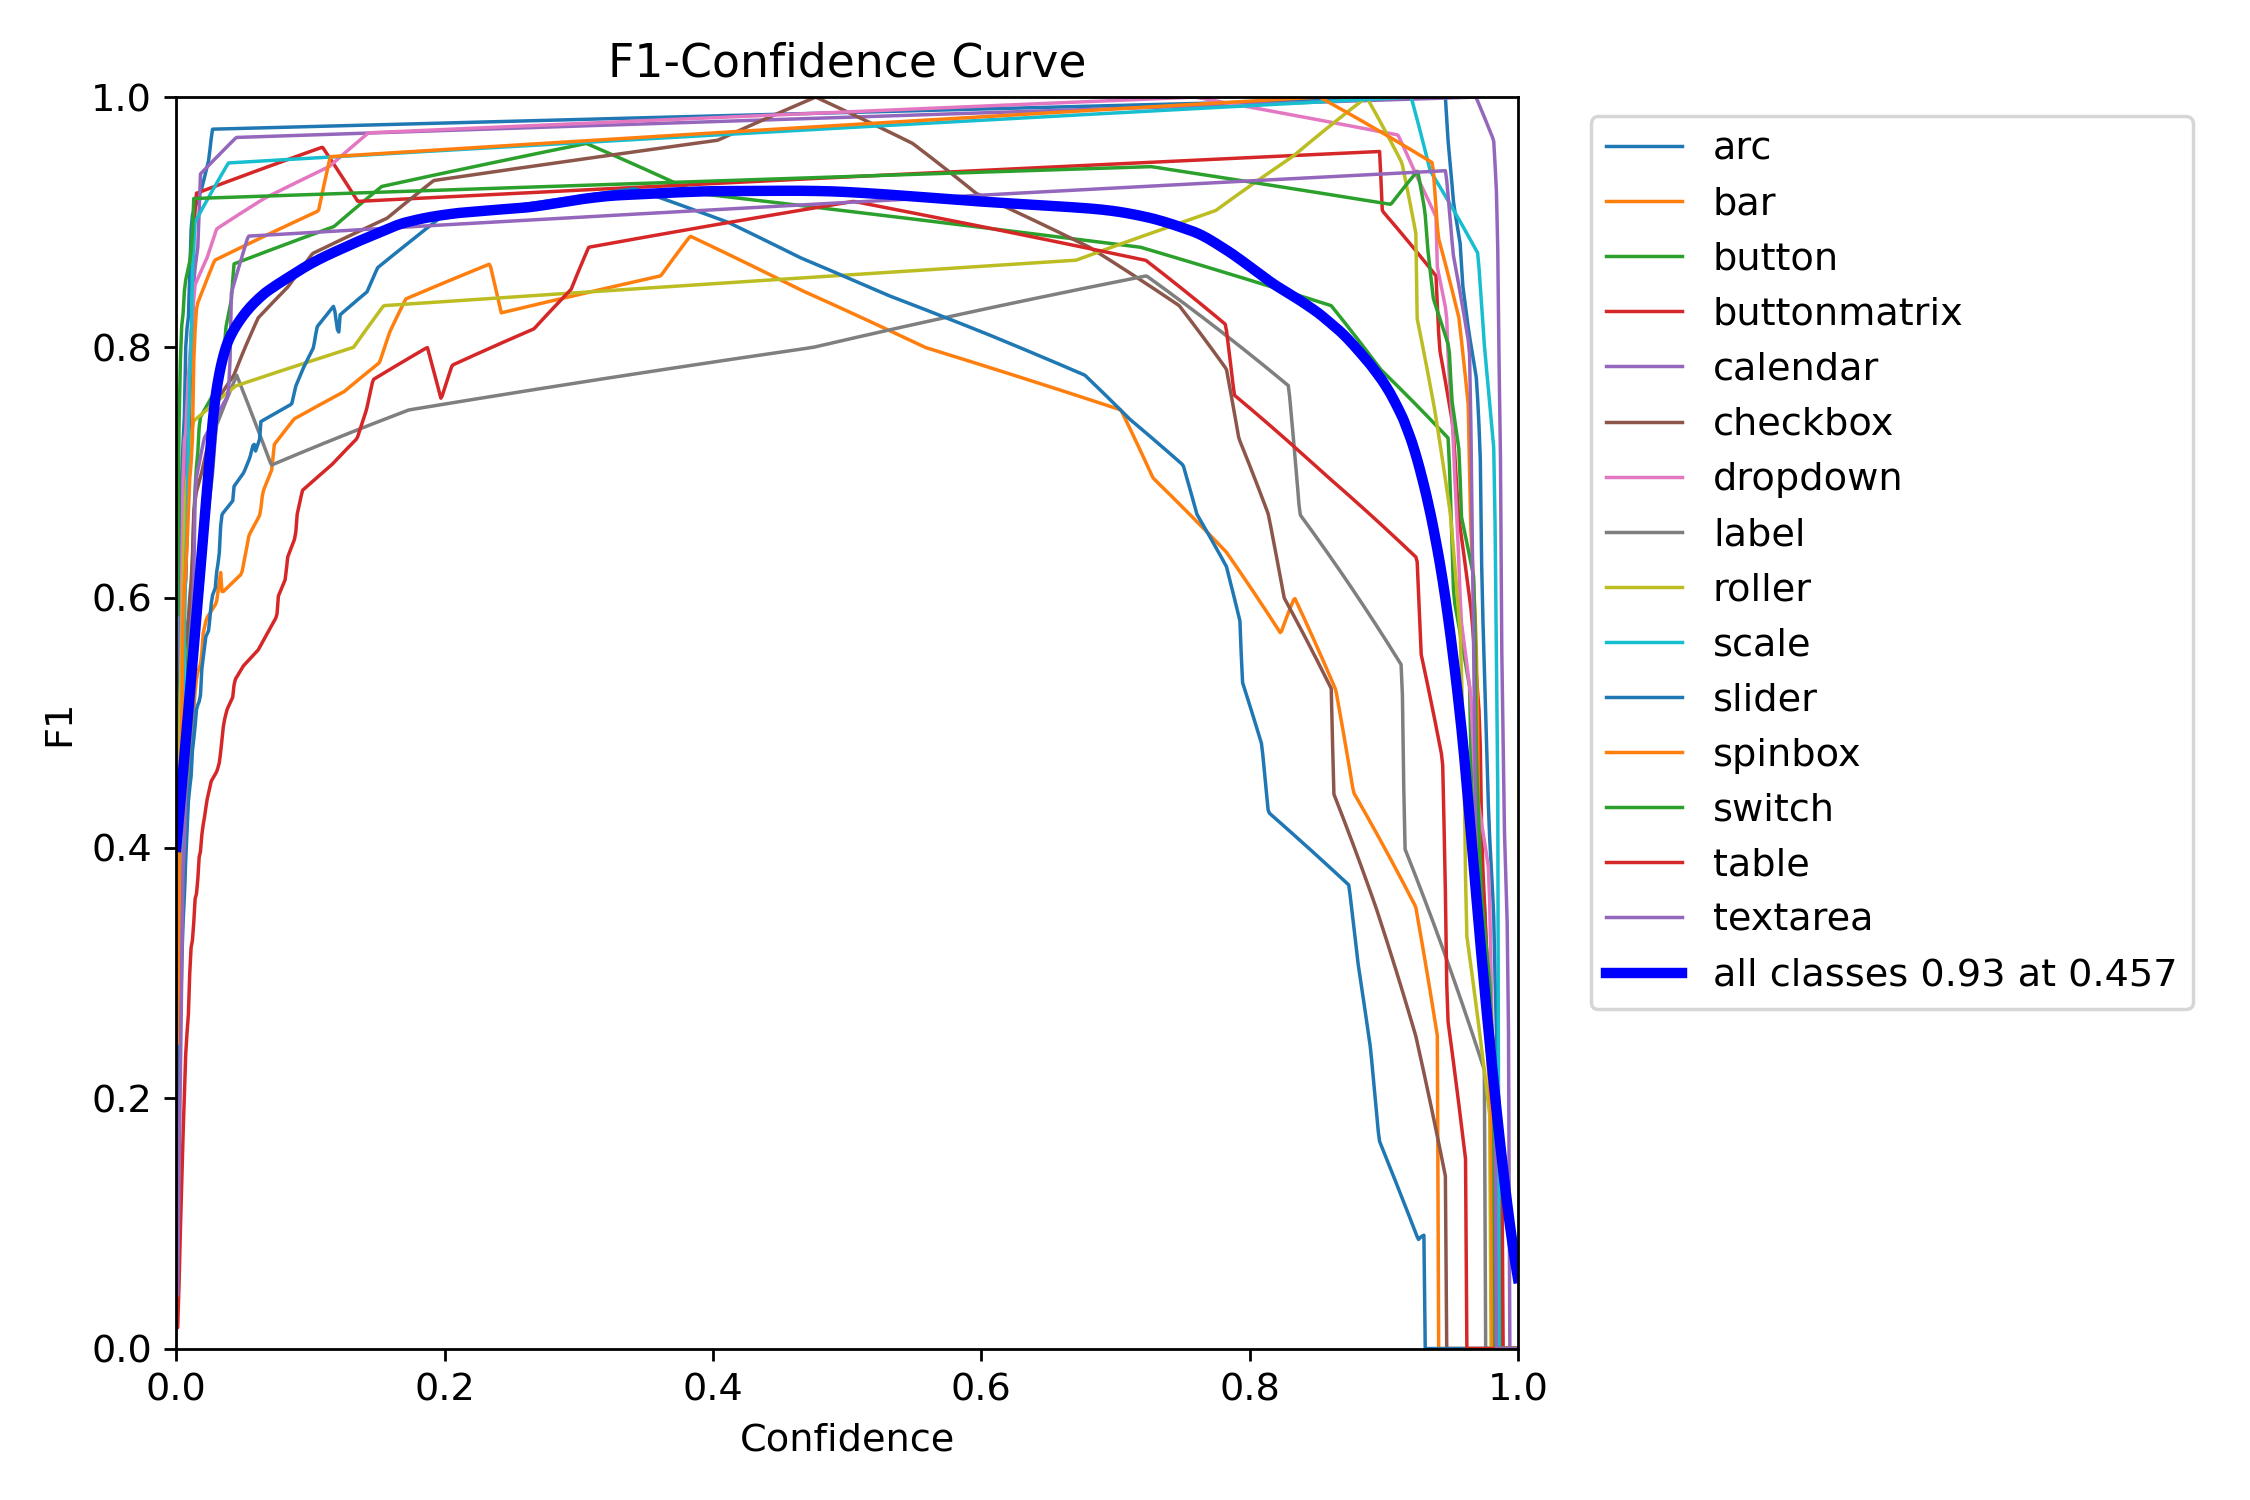
\includegraphics[width=\textwidth]{PICs/train371/F1_curve.png}
    \label{fig:random-training-f1}
\end{figure}
Further training visualizations for the design dataset are depicted in Fig.\ref{fig:design-training-results},\ref{fig:design-training-confusion},\ref{fig:design-training-labels} and \ref{fig:design-training-f1}.
\begin{figure}
    \caption{Design dataset training - results}
    \centering
    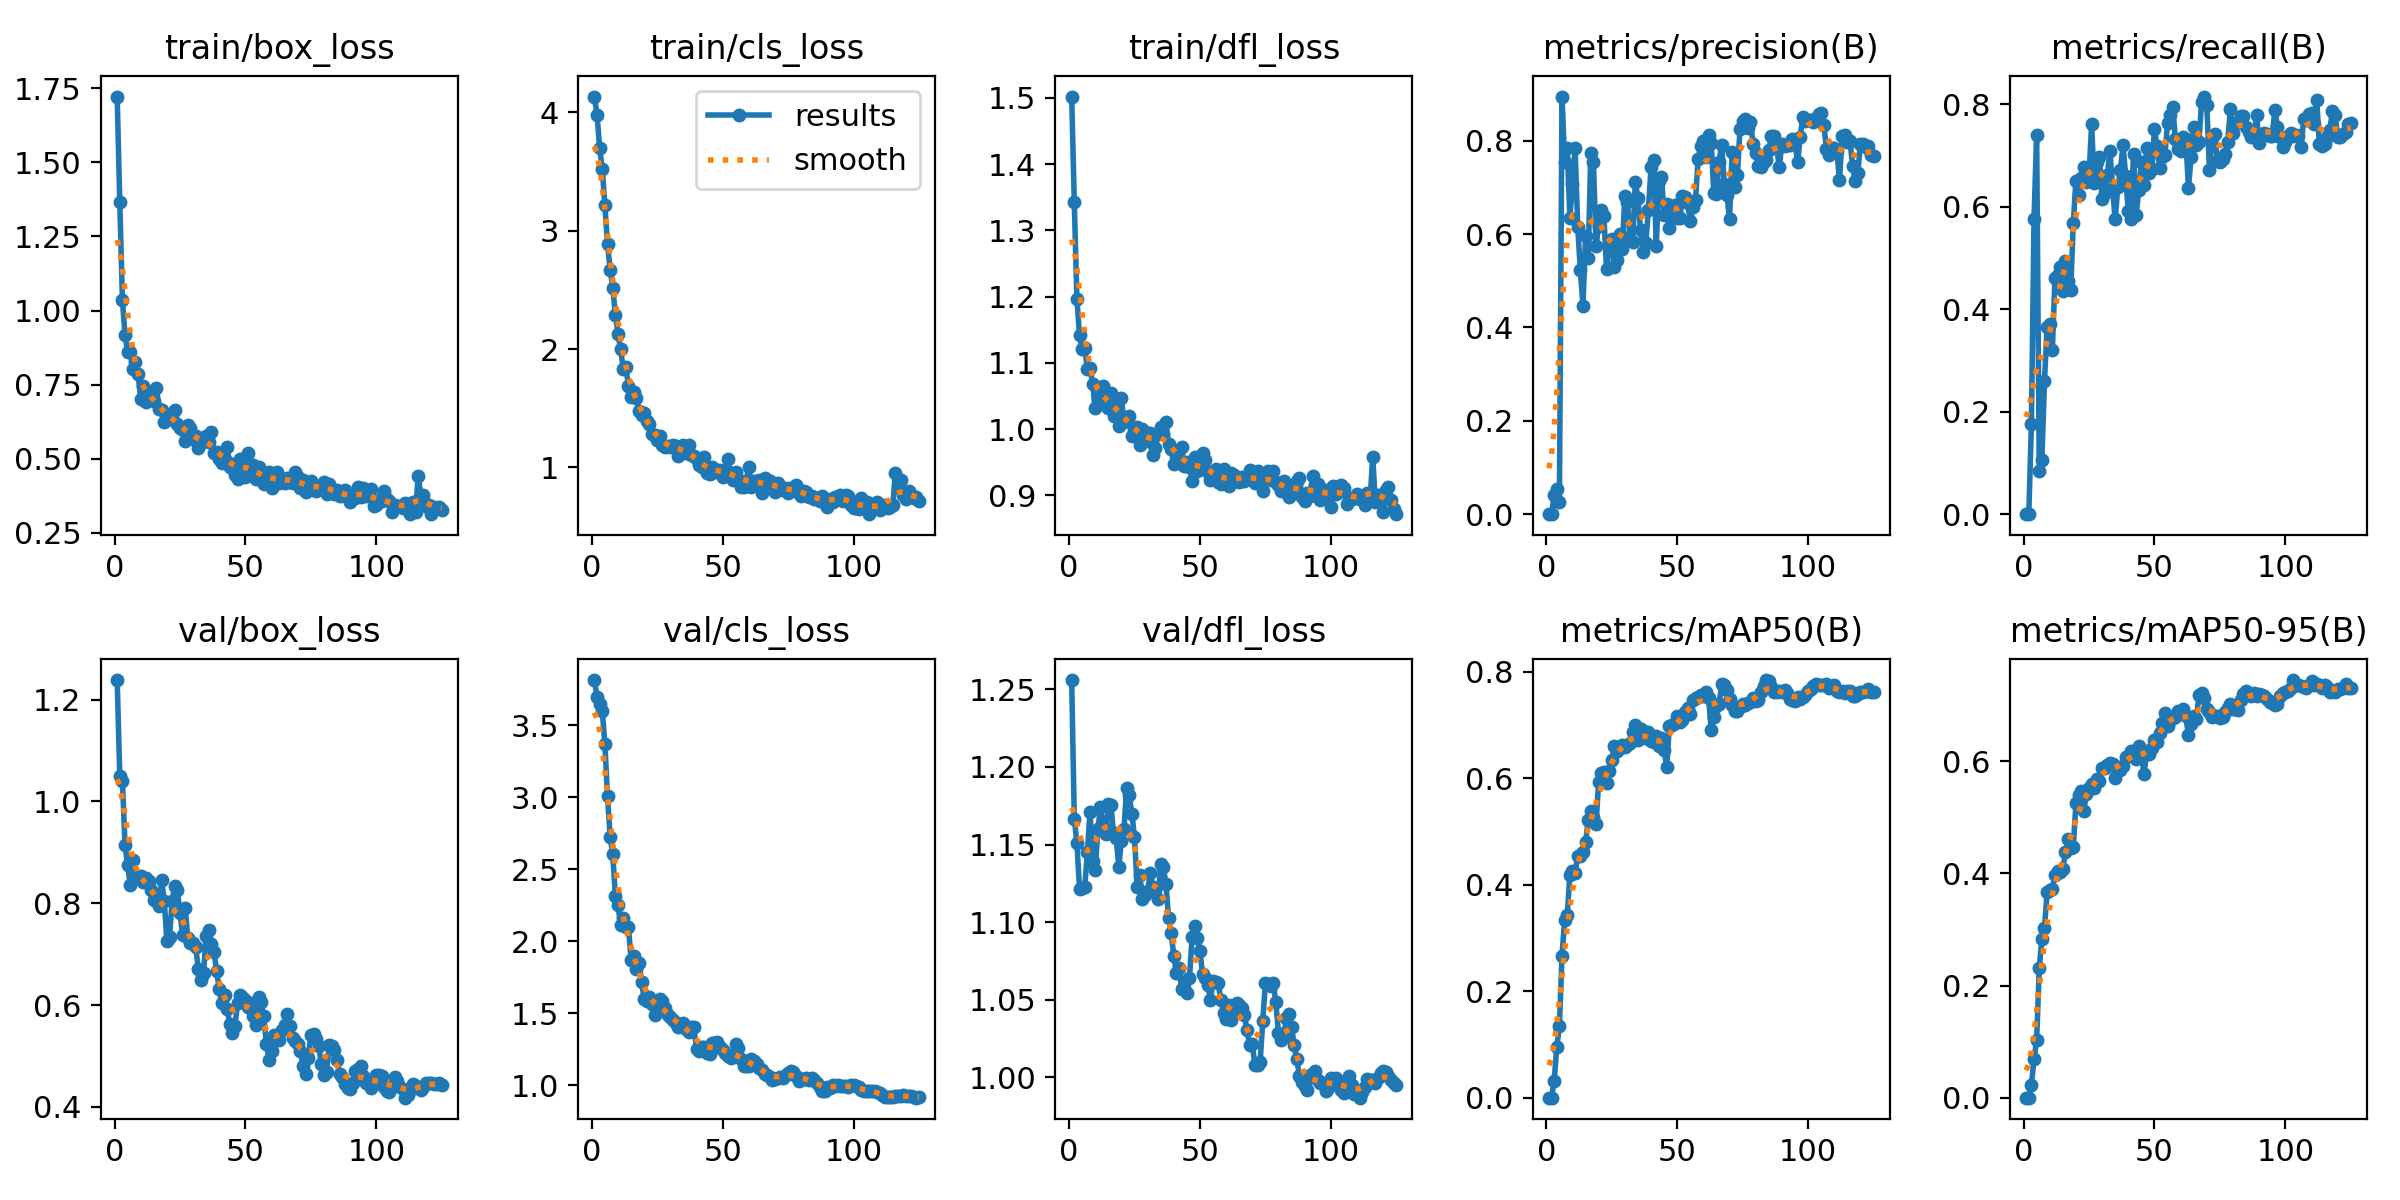
\includegraphics[width=\textwidth]{PICs/train373/results.png}
    \label{fig:design-training-results}
\end{figure}
\begin{figure}
    \caption{Design dataset training - confusion matrix (normalized)}
    \centering
    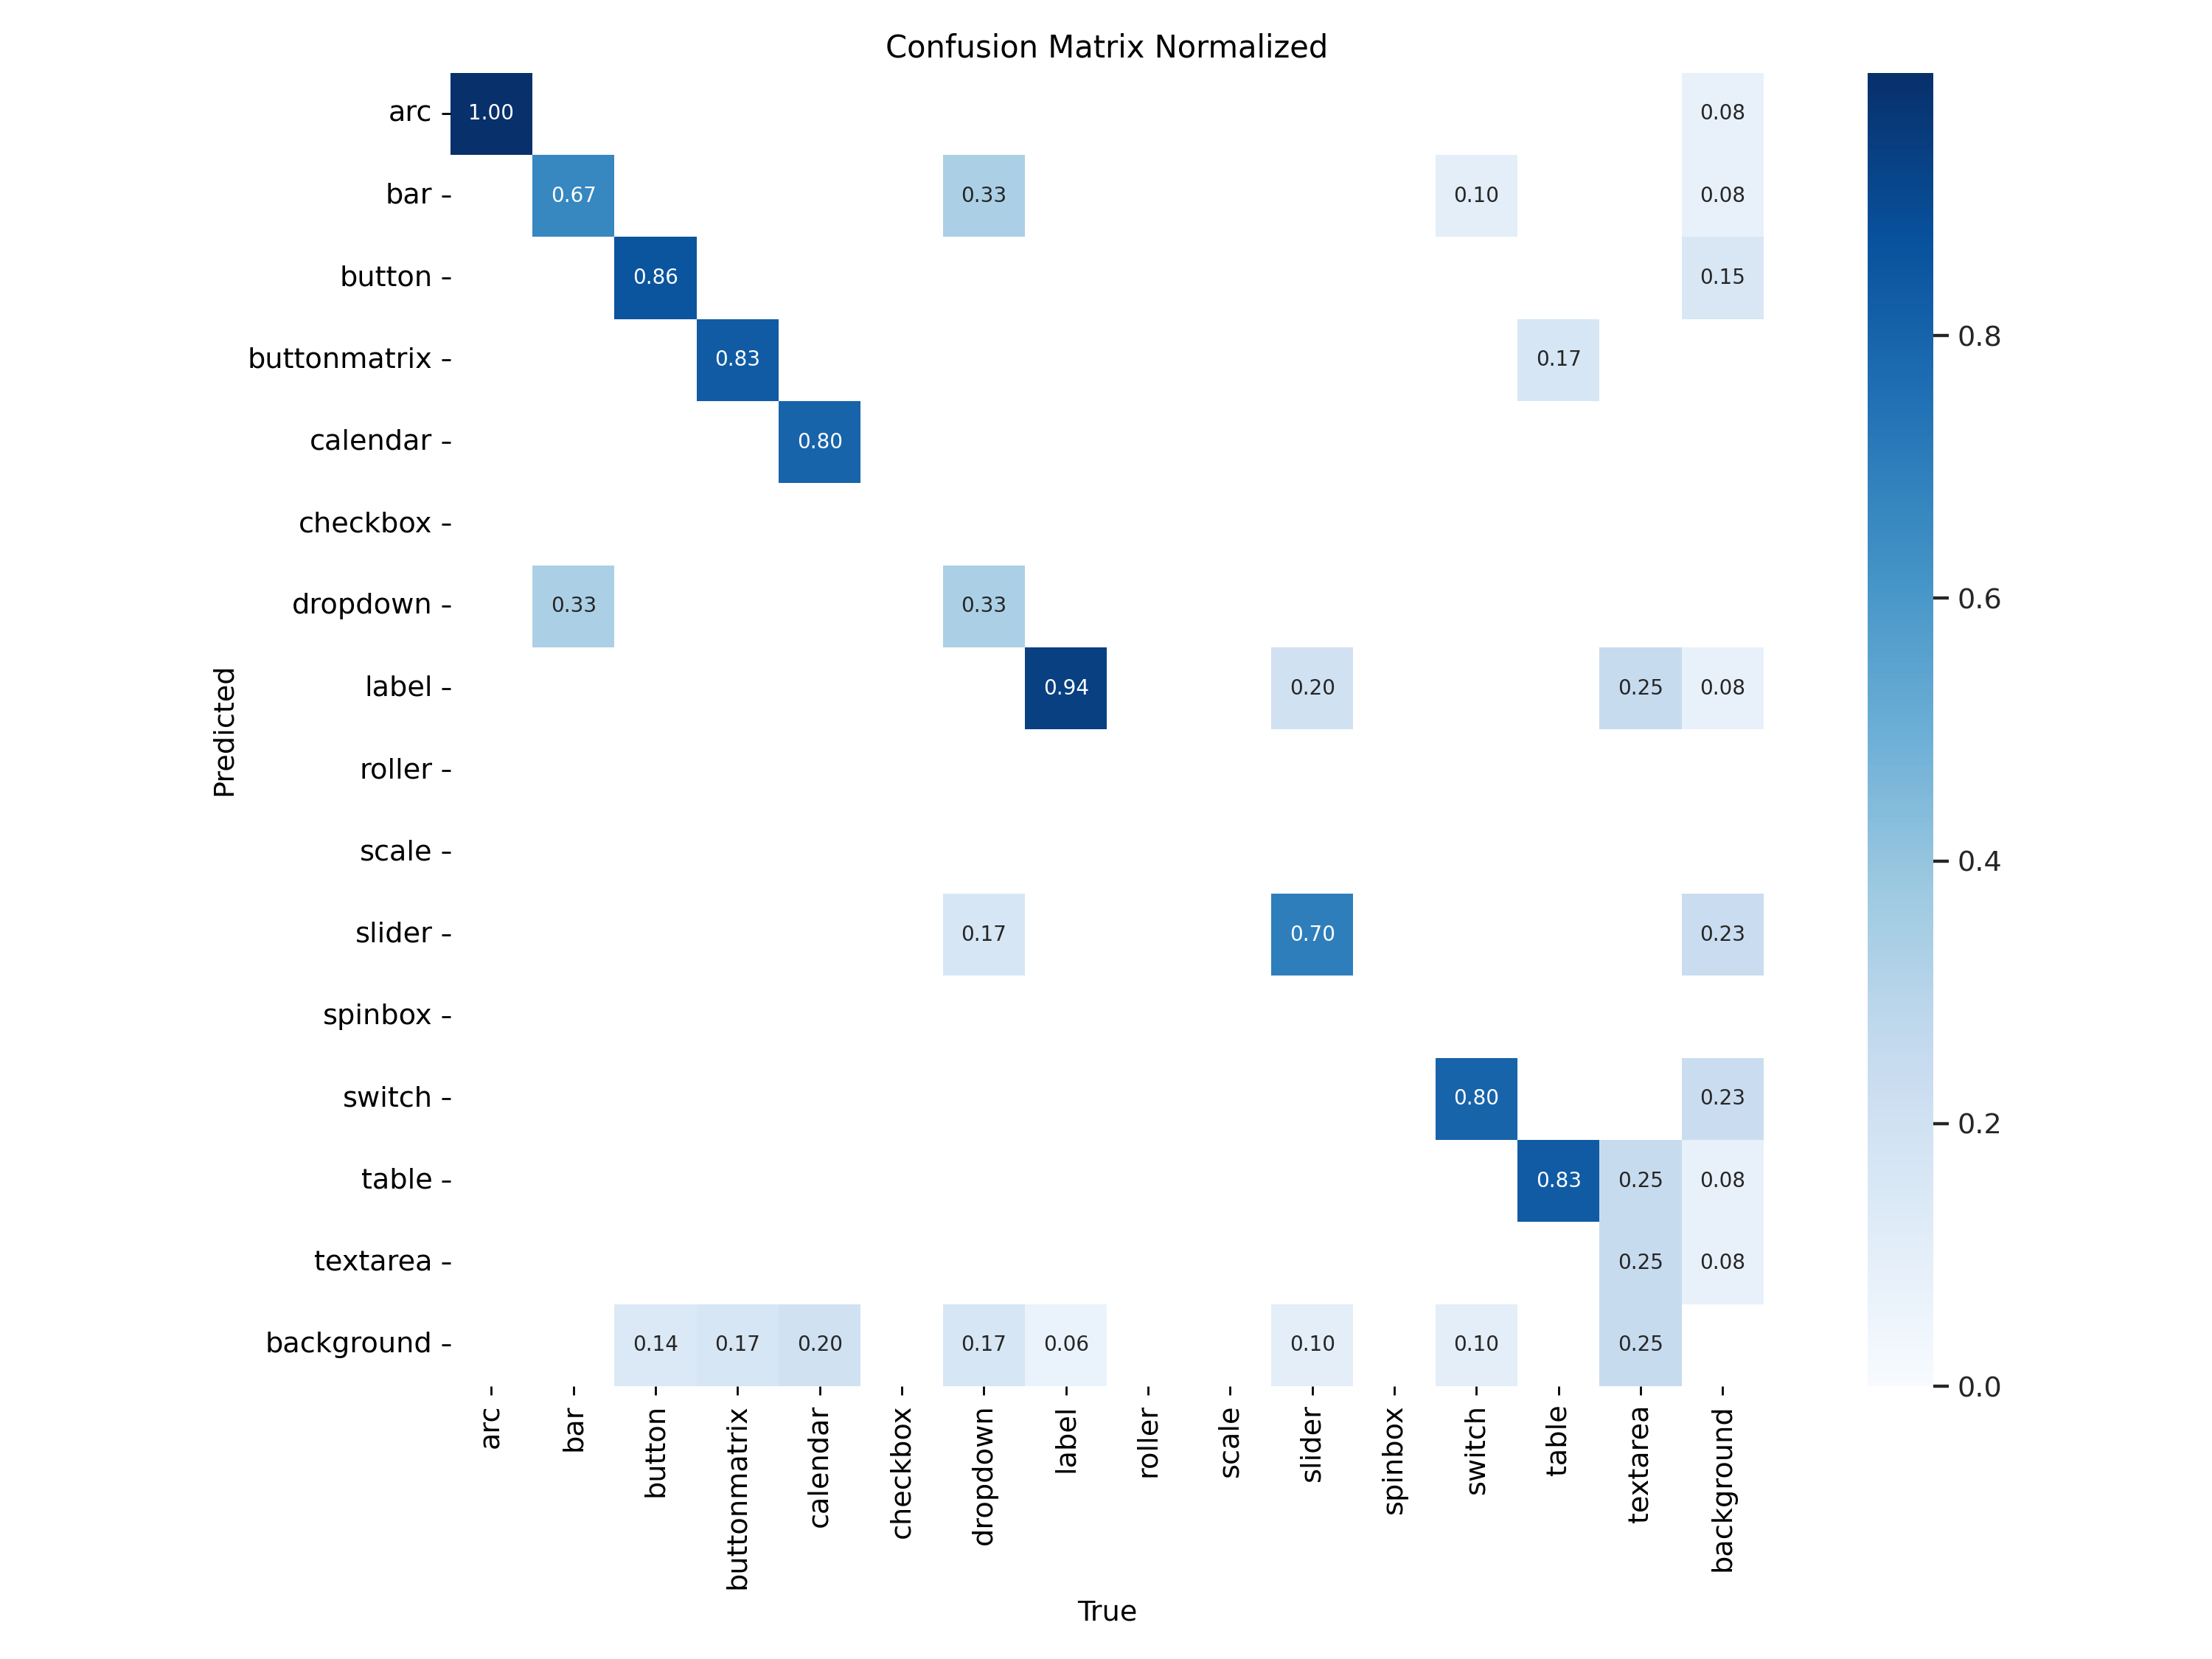
\includegraphics[width=\textwidth]{PICs/train373/confusion_matrix_normalized.png}
    \label{fig:design-training-confusion}
\end{figure}
\begin{figure}
    \caption{Design dataset training - label distribution}
    \centering
    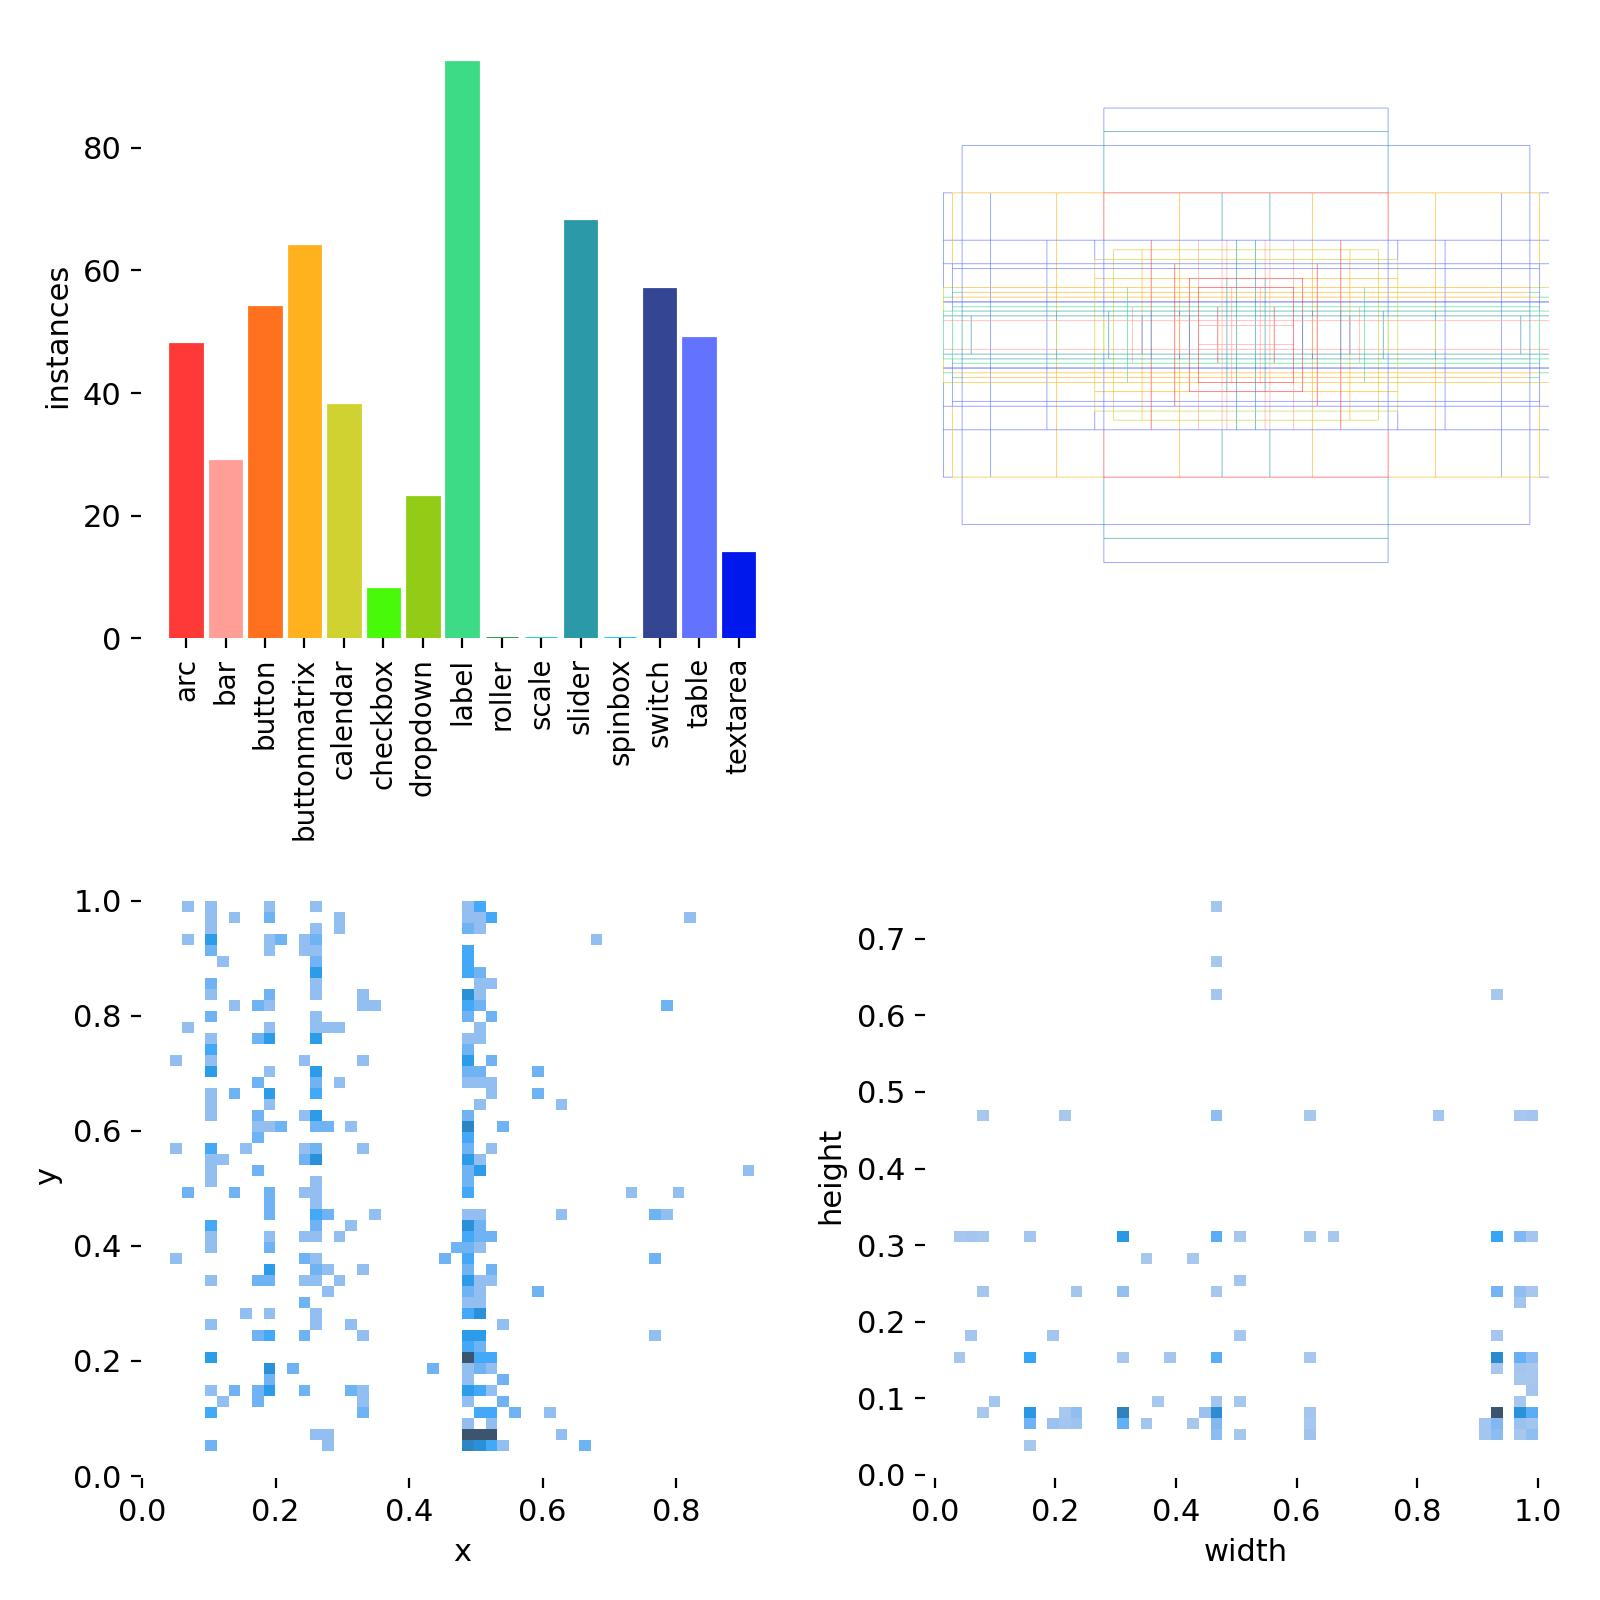
\includegraphics[width=\textwidth]{PICs/train373/labels.jpg}
    \label{fig:design-training-labels}
\end{figure}
\begin{figure}
    \caption{Design dataset training - F1 curve}
    \centering
    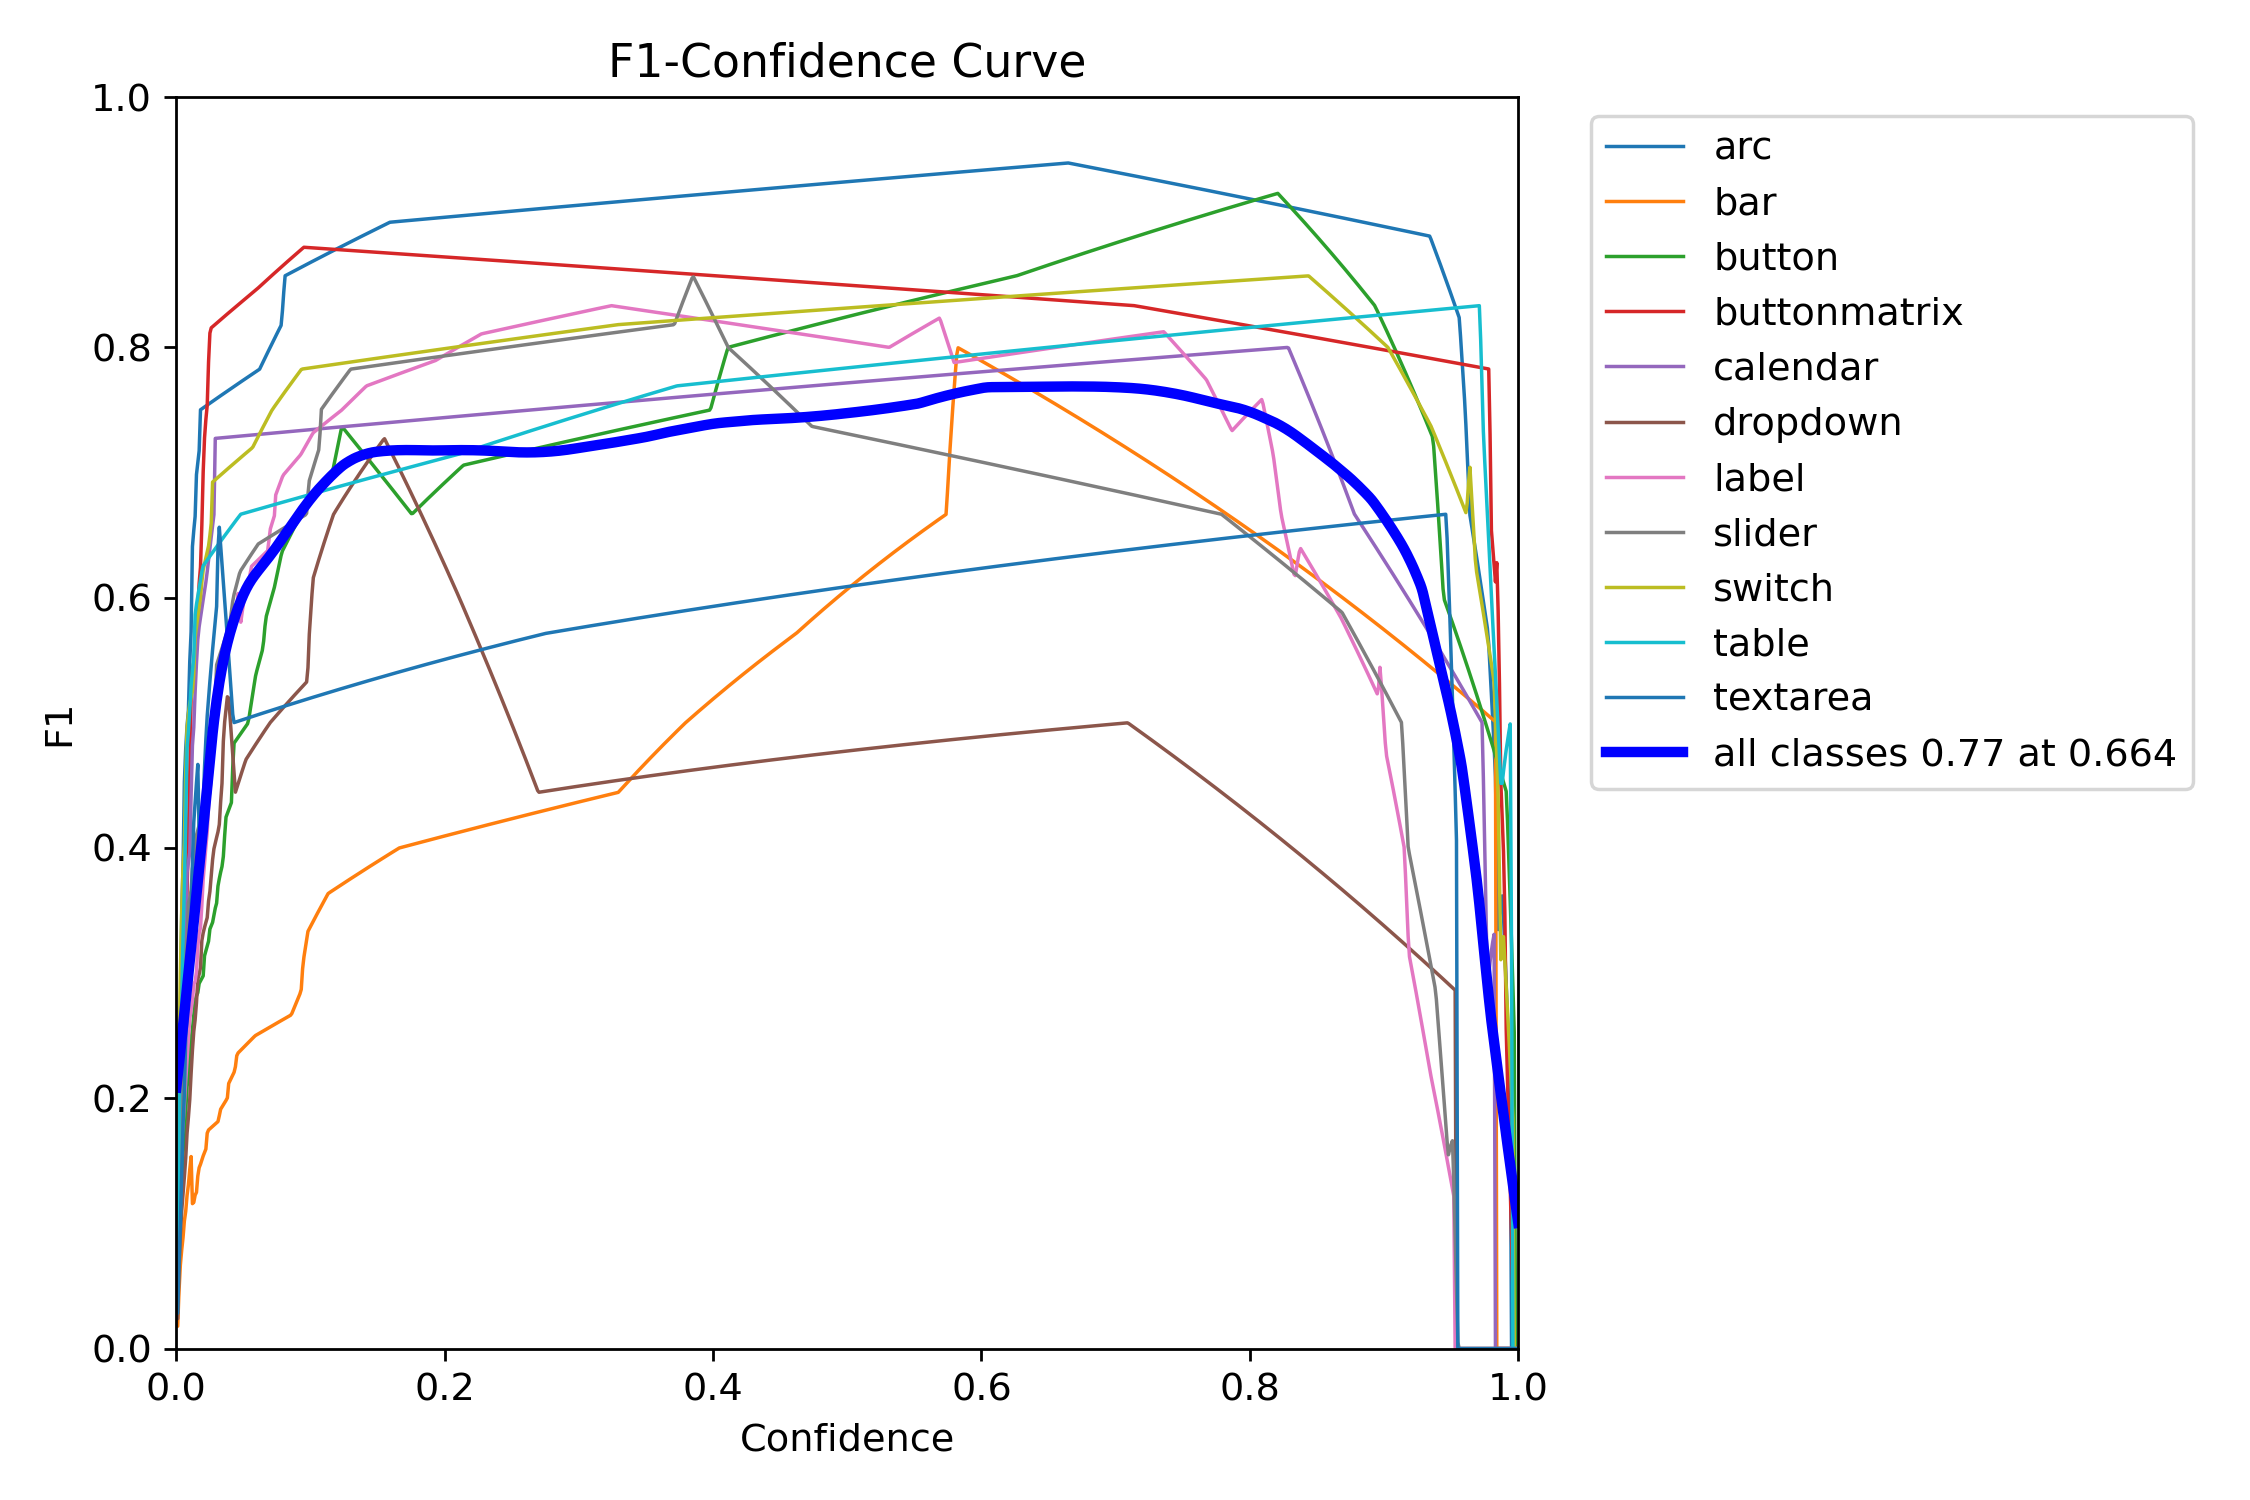
\includegraphics[width=\textwidth]{PICs/train373/F1_curve.png}
    \label{fig:design-training-f1}
\end{figure}
\clearpage
\subsection{Random based dataset}
The used random dataset contains 15 different widget types of \ac{lvgl} in varying positions and widget styles (excluding container style), where each widget is represented about 150 times, as showcased in Fig.\ref{fig:random-widget-metrics}. The total amount of widgets in the dataset is 2250, spread over 406 image files.\\
\begin{figure}
    \caption{Generator v2 iteration metrics for random dataset}
    \centering
    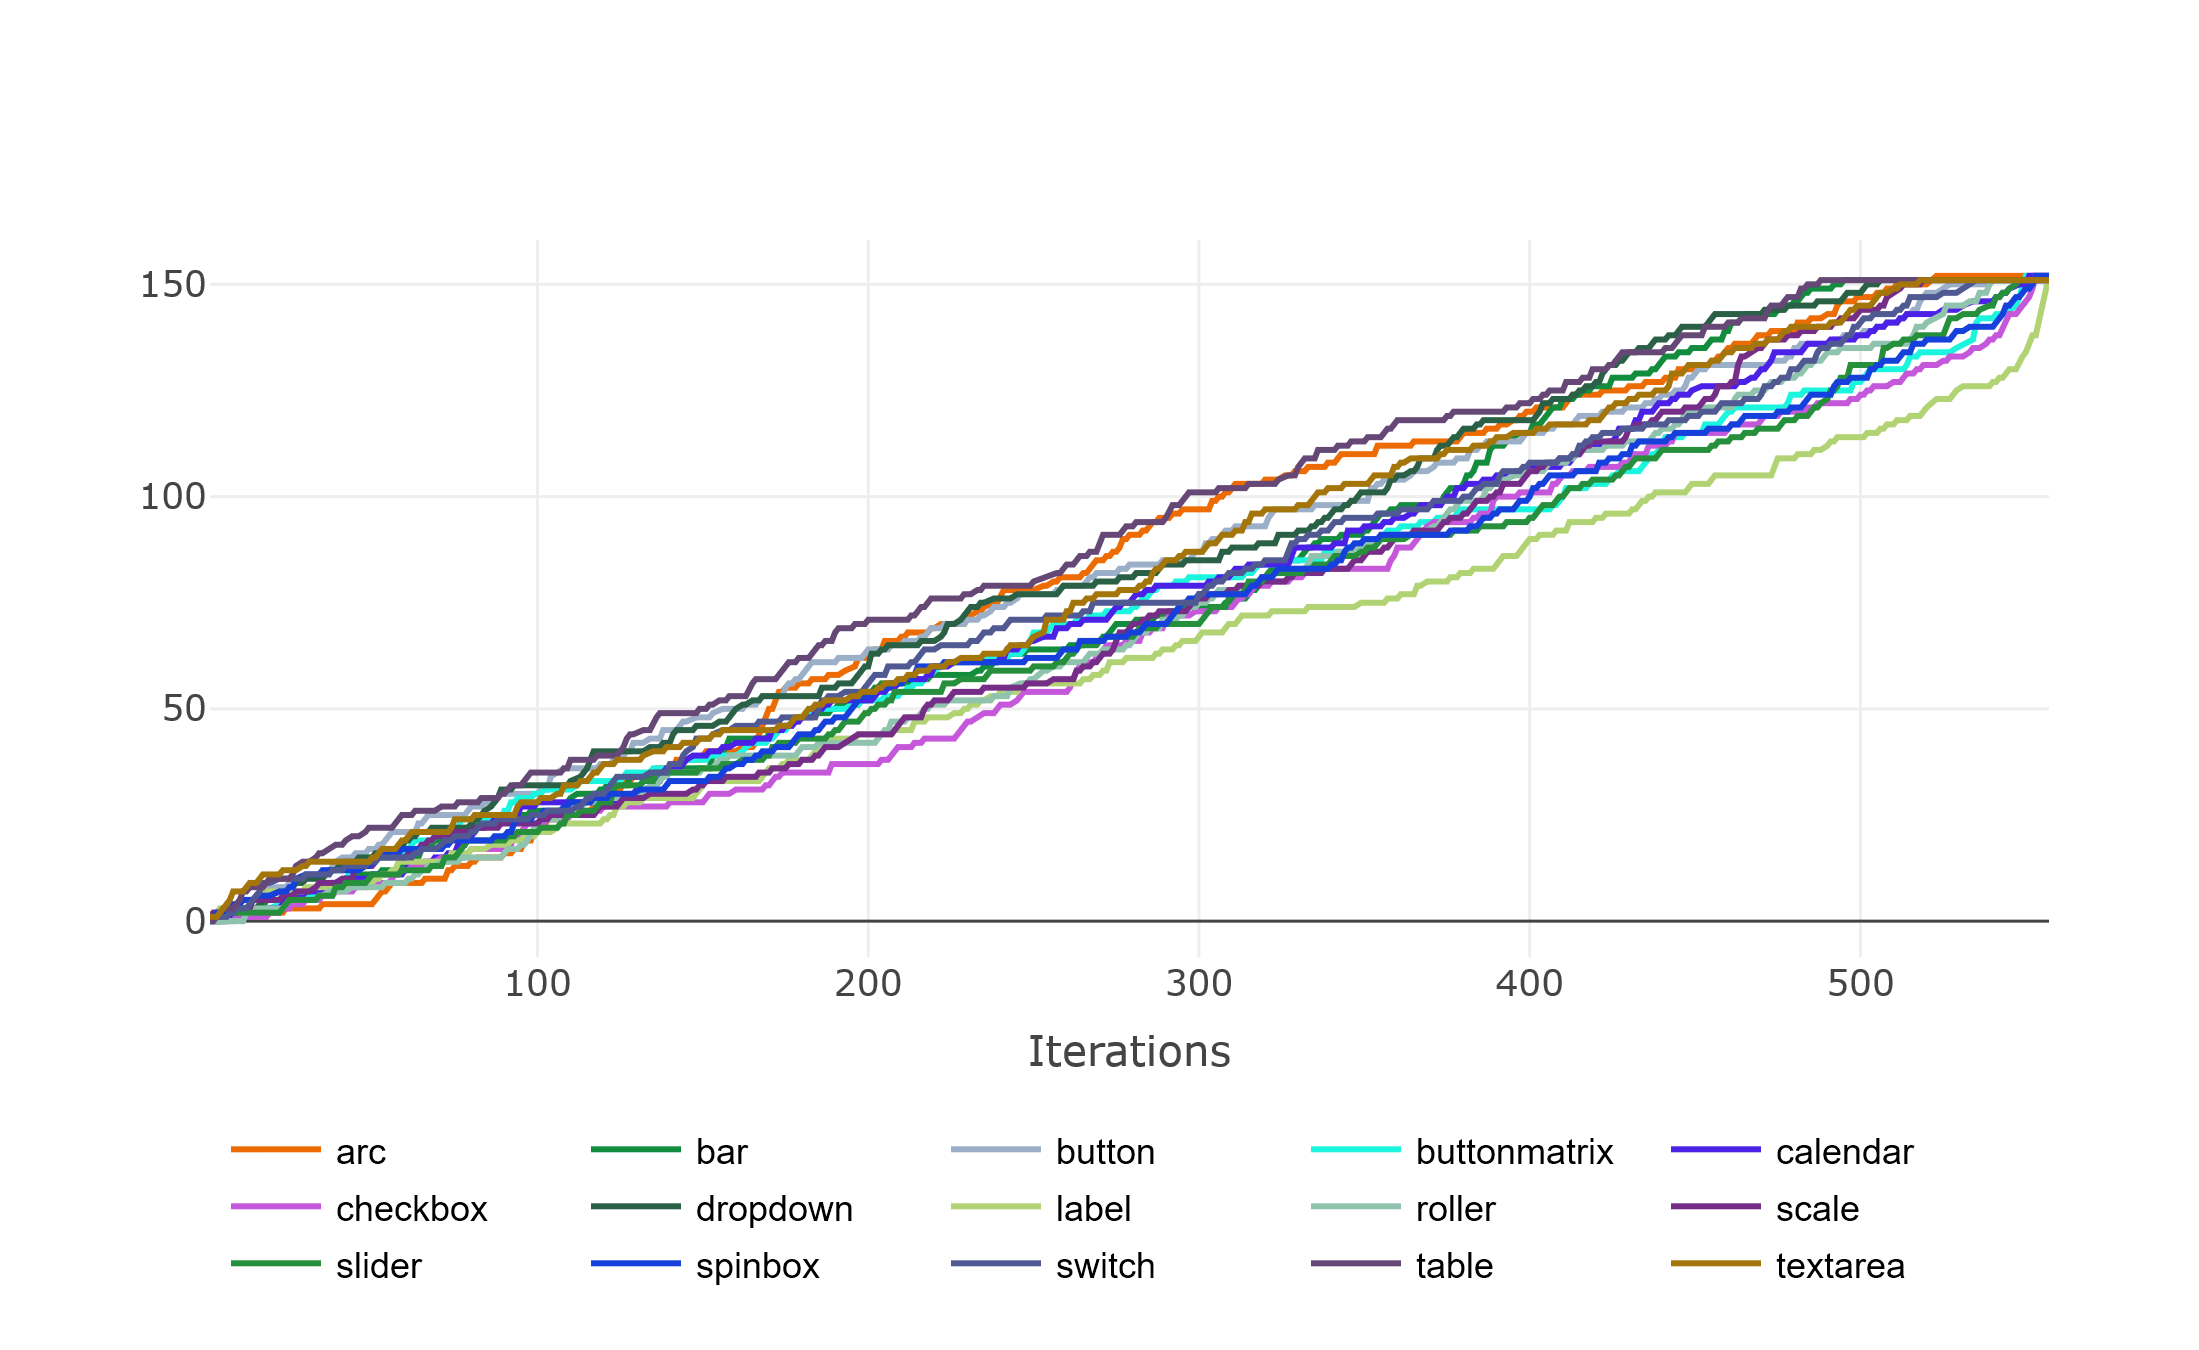
\includegraphics[width=\textwidth]{random_widget_metrics.png}
    \label{fig:random-widget-metrics}
\end{figure}
In the dataset, each image contained 6 widget instances. The dataset is uploaded to the repository of the paper \autocite{ReleaseFinalPaper} and can be referenced by ID \code{04da75baa7084aee83f3b31602c408c2}.
\subsection{Design based dataset}
The design dataset has 145 design files. Not all designs could be generated, so only an output of 132 generated images was achieved. Due to the described distortion issue in the generator, the dataset had to be manually corrected by removing broken images and adding in replacements of other design generations. The corrected design dataset contains 186 images.\\
Since the process of adding in images was performed manually, an exact widget count cannot be given, but is estimated to contain roughly 550 widgets. In Fig.\ref{fig:design-training-labels} the label distribution of the dataset can be seen.\\
Certain widget types were definitely more preferred by the \ac{llm}, while three (roller, scale, spinbox) are not represented at all. For the design mode it is inherently more difficult to create a balance in distribution, as certain widget types like buttons or labels will always be over-represented when trying to create realistic looking \ac{ui}.
The original design dataset with some image distortions is referenced by ID \code{5c8e248bdcc24ee2bb57760f0961c690}. The manually corrected version is referenced by ID \code{2fe5e8b06a6249fcb9360c9645e0f7a6}. Both are uploaded to the repository of the paper \autocite{ReleaseFinalPaper}.
\section{Impact of style variation}
An important factor discovered during the research is the importance of style variation when training a \ac{yolo} model on \ac{ui} image data. Given that in the real-world \acp{ui} need to appeal to humans and also be usable by them, it is important to incorporate style variations into training datasets. This avoids over-optimized datasets illustrating best-case detection scenarios where individual widget features would be more easily detected by the model. Incorporating themes and contexts into artificially generated \ac{ui} brings the benefit of creating datasets, that are more aligned with worst-case detection scenarios, where individual widgets need to be differentiated with better precision. It is recommended to experiment with outlines and other style properties when creating such datasets and training future models in the context of \ac{ui} widget detection.
%%%%%%%%%%%%%%%%%%%%%%%%%%%%%%%%%%%%%%%% Start of discussion
\chapter{Discussion}
While the results of the model on the synthesized datasets looks promising, they are far from being usable when used on real data. The output models of both final runs were used in a prediction test against design mock-ups of a new \ac{ui} design. This test showcased that the models perform much worse or not at all when faced with unseen complexity in widget style, nested widgets, used symbols and fonts. In the test, both models were not able to properly predict all widgets. The most promising type in those test results was the button, which was not only often correctly identified but also with a much higher confidence than the rest. One has to keep in mind that these proprietary designs are far more advanced than what the generator could provide, which means that that further development and refinement in the generation process would be necessary, in order for the models to deliver better performance. Due to company secrets, it was not possible to showcase those test images in the thesis.\\
In regards to the stated research questions the viability of the \ac{ml} object detection approach is reasonably possible, but a definitive answer cannot be given as the initial test on a real user interface was a failure. Further development in the created generators is necessary, which will be conducted at the discretion of Schrack Seconet.
%%%%%%%%%%%%%%%%%%%%%%%%%%%%%%%%%%%%%%%%%%%%%%%%%%%%%%%%%%%%%% End of content
%%%%%%%%%%%%%%%%%%%%%%%%%%%%%%%%%%%%%%%%%%%%%%%%%%%%%%%%%%%%%% Start of listings
\clearpage % Beginne neue Seite

\printbibliography
%\printbib % Literaturverzeichnis LaTeX-Zitier-Standard
%\printbib{Literature}                                             % Literaturverzeichnis FH-Zitier-Standard
\clearpage

\listoffigures % Abbildungsverzeichnis
\clearpage

\listoftables % Tabellenverzeichnis
\clearpage

\listoflistings % Quellcodeverzeichnis
\clearpage

\phantomsection
\addcontentsline{toc}{chapter}{\listacroname}
\chapter*{\listacroname}
% TODO REMOVE UNUSED ACRONYMS AT THE END OF WRITING
\begin{acronym}
    % \acro{api}[API]{Application Programming Interface}
    % \acro{yoloAlt}[YOLO]{You only live once}
    % \acro{yolo}[YOLO]{You Only Look Once}
    % \acro{yolo8}[YOLOv8]{YOLO version 8 by ultralytics}
    % \acro{ui}[UI]{user interface}
    % \acro{gui}[GUI]{graphical user interface}
    % \acro{ta}[TA]{test automation}
    % \acro{sut}[SUT]{system under test}
    % \acro{json}[JSON]{JavaScript Object Notation}
    % \acro{cli}[CLI]{Command-line interface}
    % \acro{mcu}[MCU]{Microcontroller unit}
    % \acro{led}[LED]{Light Emitting Diode}
    % \acro{lvgl}[LVGL]{Light and versatile graphics library}
    % \acro{fas}[FAS]{fire alarm system}
    % \acro{hcs}[HCS]{health care system}
    % \acro{ml}[ML]{machine learning}
    % \acro{hpo}[HPO]{hyper-parameter optimization}
    % \acro{iou}[IoU]{Intersection over Union}
    % \acro{map}[mAP]{mean average precision}
    % \acro{llm}[LLM]{large language model}
    % \acro{gpt}[GPT]{generative pre-trained transformer}
    % \acro{cnn}[CNN]{Convolutional Neural Network}
    % \acro{vcip}[VCIP]{Visocall IP}
    % \acro{vgt}[VGT]{visual GUI testing}
    \acro{api}[API]{Application Programming Interface}
    \acro{cli}[CLI]{Command-line interface}
    \acro{cnn}[CNN]{Convolutional Neural Network}
    \acro{fas}[FAS]{fire alarm system}
    \acro{gpt}[GPT]{generative pre-trained transformer}
    \acro{gui}[GUI]{graphical user interface}
    \acro{hcs}[HCS]{health care system}
    \acro{hpo}[HPO]{hyper-parameter optimization}
    \acro{iou}[IoU]{Intersection over Union}
    \acro{json}[JSON]{JavaScript Object Notation}
    \acro{led}[LED]{Light Emitting Diode}
    \acro{llm}[LLM]{large language model}
    \acro{lvgl}[LVGL]{Light and versatile graphics library}
    \acro{map}[mAP]{mean average precision}
    \acro{mcu}[MCU]{Microcontroller unit}
    \acro{ml}[ML]{machine learning}
    \acro{sut}[SUT]{system under test}
    \acro{ta}[TA]{test automation}
    \acro{vcip}[VCIP]{Visocall IP}
    \acro{vgt}[VGT]{visual GUI testing}
    \acro{ui}[UI]{user interface}
    \acro{yoloAlt}[YOLO]{You only live once}
    \acro{yolo}[YOLO]{You Only Look Once}
    \acro{yolo8}[YOLOv8]{YOLO version 8 by ultralytics}
\end{acronym}
%%%%%%%%%%%%%%%%%%%%%%%%%%%%%%%%%%%%%%%%%%%%%%%%%%%%%%%%%%%%%%%%%% End of listings
%%%%%%%%%%%%%%%%%%%%%%%%%%%%%%%%%%%%%%%%%%%%%%%%%%%%%%%%%%%%%%%%%% Start of appendix
% \clearpage
% \appendix
% \clearpage
\end{document}
%%%%%%%%%%%%%%%%%%%%%%%%%%%%%%%%%%%%%%%%%%%%%%%%%%%%%%%%%%%%%%%%%% End of appendix